\documentclass[]{report}
\usepackage{tikz}
\usepackage{listings}
\usepackage{color}

\definecolor{dkgreen}{rgb}{0,0.6,0}
\definecolor{gray}{rgb}{0.5,0.5,0.5}
\definecolor{mauve}{rgb}{0.58,0,0.82}
%opening
\title{SY19}
\author{}

\begin{document}
	
\lstset{frame=tb,
	language=R,
	aboveskip=3mm,
	belowskip=3mm,
	showstringspaces=false,
	columns=flexible,
	basicstyle={\small\ttfamily},
	numbers=none,
	numberstyle=\tiny\color{gray},
	keywordstyle=\color{blue},
	commentstyle=\color{dkgreen},
	stringstyle=\color{mauve},
	breaklines=true,
	breakatwhitespace=true,
	tabsize=3
}

\maketitle

\part{Abreviations}
	

\begin{abstract}

\end{abstract}

\part{Introduction}

\part{Ex 1}

\part{Ex 2 - Breast Cancer Recurring Time}

\section{Introduction}
This part aims to build the best model to predict the recurring time of breast cancer based on about 30 features computed from a breast mass.  This regression problem will take advantage of a given dataset describing about 200 patient cases.

\section{Dataset Description}
We take a look at the raw dataset to get first hints on how each feature contributes to the recurring time.

The dataset comprises 194 patient cases, each of which is described through 32 features and the cancer recurring time \texttt{Time} that we have to predict.

\subsection{Time}
Let's first describe the evolution of the variable \texttt{Time}. To do so, we can use the R functions \texttt{boxplot} and \texttt{hist}.

\begin{figure}[!hb]
	\centering
	% Created by tikzDevice version 0.10.1 on 2016-11-19 14:20:25
% !TEX encoding = UTF-8 Unicode
\begin{tikzpicture}[x=1pt,y=1pt]
\definecolor{fillColor}{RGB}{255,255,255}
\path[use as bounding box,fill=fillColor,fill opacity=0.00] (0,0) rectangle (505.89,505.89);
\begin{scope}
\path[clip] ( 49.20, 61.20) rectangle (480.69,456.69);
\definecolor{drawColor}{RGB}{0,0,0}

\path[draw=drawColor,line width= 1.2pt,line join=round] (185.04,189.55) -- (344.85,189.55);

\path[draw=drawColor,line width= 0.4pt,dash pattern=on 4pt off 4pt ,line join=round,line cap=round] (264.94, 75.85) -- (264.94,114.24);

\path[draw=drawColor,line width= 0.4pt,dash pattern=on 4pt off 4pt ,line join=round,line cap=round] (264.94,442.04) -- (264.94,288.48);

\path[draw=drawColor,line width= 0.4pt,line join=round,line cap=round] (224.99, 75.85) -- (304.90, 75.85);

\path[draw=drawColor,line width= 0.4pt,line join=round,line cap=round] (224.99,442.04) -- (304.90,442.04);

\path[draw=drawColor,line width= 0.4pt,line join=round,line cap=round] (185.04,114.24) --
	(344.85,114.24) --
	(344.85,288.48) --
	(185.04,288.48) --
	(185.04,114.24);
\end{scope}
\begin{scope}
\path[clip] (  0.00,  0.00) rectangle (505.89,505.89);
\definecolor{drawColor}{RGB}{0,0,0}

\path[draw=drawColor,line width= 0.4pt,line join=round,line cap=round] ( 49.20, 72.89) -- ( 49.20,427.28);

\path[draw=drawColor,line width= 0.4pt,line join=round,line cap=round] ( 49.20, 72.89) -- ( 43.20, 72.89);

\path[draw=drawColor,line width= 0.4pt,line join=round,line cap=round] ( 49.20,131.96) -- ( 43.20,131.96);

\path[draw=drawColor,line width= 0.4pt,line join=round,line cap=round] ( 49.20,191.02) -- ( 43.20,191.02);

\path[draw=drawColor,line width= 0.4pt,line join=round,line cap=round] ( 49.20,250.09) -- ( 43.20,250.09);

\path[draw=drawColor,line width= 0.4pt,line join=round,line cap=round] ( 49.20,309.15) -- ( 43.20,309.15);

\path[draw=drawColor,line width= 0.4pt,line join=round,line cap=round] ( 49.20,368.21) -- ( 43.20,368.21);

\path[draw=drawColor,line width= 0.4pt,line join=round,line cap=round] ( 49.20,427.28) -- ( 43.20,427.28);

\node[text=drawColor,rotate= 90.00,anchor=base,inner sep=0pt, outer sep=0pt, scale=  1.00] at ( 34.80, 72.89) {0};

\node[text=drawColor,rotate= 90.00,anchor=base,inner sep=0pt, outer sep=0pt, scale=  1.00] at ( 34.80,131.96) {20};

\node[text=drawColor,rotate= 90.00,anchor=base,inner sep=0pt, outer sep=0pt, scale=  1.00] at ( 34.80,191.02) {40};

\node[text=drawColor,rotate= 90.00,anchor=base,inner sep=0pt, outer sep=0pt, scale=  1.00] at ( 34.80,250.09) {60};

\node[text=drawColor,rotate= 90.00,anchor=base,inner sep=0pt, outer sep=0pt, scale=  1.00] at ( 34.80,309.15) {80};

\node[text=drawColor,rotate= 90.00,anchor=base,inner sep=0pt, outer sep=0pt, scale=  1.00] at ( 34.80,368.21) {100};

\node[text=drawColor,rotate= 90.00,anchor=base,inner sep=0pt, outer sep=0pt, scale=  1.00] at ( 34.80,427.28) {120};

\path[draw=drawColor,line width= 0.4pt,line join=round,line cap=round] ( 49.20, 61.20) --
	(480.69, 61.20) --
	(480.69,456.69) --
	( 49.20,456.69) --
	( 49.20, 61.20);
\end{scope}
\end{tikzpicture}

	\caption{Box Plot}
\end{figure}

\begin{figure}[!hb]
	\centering
	% Created by tikzDevice version 0.10.1 on 2016-11-19 14:20:58
% !TEX encoding = UTF-8 Unicode
\begin{tikzpicture}[x=1pt,y=1pt]
\definecolor{fillColor}{RGB}{255,255,255}
\path[use as bounding box,fill=fillColor,fill opacity=0.00] (0,0) rectangle (505.89,505.89);
\begin{scope}
\path[clip] (  0.00,  0.00) rectangle (505.89,505.89);
\definecolor{drawColor}{RGB}{0,0,0}

\node[text=drawColor,anchor=base,inner sep=0pt, outer sep=0pt, scale=  1.00] at (264.94, 15.60) {Time};

\node[text=drawColor,rotate= 90.00,anchor=base,inner sep=0pt, outer sep=0pt, scale=  1.00] at ( 10.80,258.94) {Time};
\end{scope}
\begin{scope}
\path[clip] (  0.00,  0.00) rectangle (505.89,505.89);
\definecolor{drawColor}{RGB}{0,0,0}

\path[draw=drawColor,line width= 0.4pt,line join=round,line cap=round] ( 65.18, 61.20) -- (433.98, 61.20);

\path[draw=drawColor,line width= 0.4pt,line join=round,line cap=round] ( 65.18, 61.20) -- ( 65.18, 55.20);

\path[draw=drawColor,line width= 0.4pt,line join=round,line cap=round] (126.65, 61.20) -- (126.65, 55.20);

\path[draw=drawColor,line width= 0.4pt,line join=round,line cap=round] (188.11, 61.20) -- (188.11, 55.20);

\path[draw=drawColor,line width= 0.4pt,line join=round,line cap=round] (249.58, 61.20) -- (249.58, 55.20);

\path[draw=drawColor,line width= 0.4pt,line join=round,line cap=round] (311.04, 61.20) -- (311.04, 55.20);

\path[draw=drawColor,line width= 0.4pt,line join=round,line cap=round] (372.51, 61.20) -- (372.51, 55.20);

\path[draw=drawColor,line width= 0.4pt,line join=round,line cap=round] (433.98, 61.20) -- (433.98, 55.20);

\node[text=drawColor,anchor=base,inner sep=0pt, outer sep=0pt, scale=  1.00] at ( 65.18, 39.60) {0};

\node[text=drawColor,anchor=base,inner sep=0pt, outer sep=0pt, scale=  1.00] at (126.65, 39.60) {20};

\node[text=drawColor,anchor=base,inner sep=0pt, outer sep=0pt, scale=  1.00] at (188.11, 39.60) {40};

\node[text=drawColor,anchor=base,inner sep=0pt, outer sep=0pt, scale=  1.00] at (249.58, 39.60) {60};

\node[text=drawColor,anchor=base,inner sep=0pt, outer sep=0pt, scale=  1.00] at (311.04, 39.60) {80};

\node[text=drawColor,anchor=base,inner sep=0pt, outer sep=0pt, scale=  1.00] at (372.51, 39.60) {100};

\node[text=drawColor,anchor=base,inner sep=0pt, outer sep=0pt, scale=  1.00] at (433.98, 39.60) {120};

\path[draw=drawColor,line width= 0.4pt,line join=round,line cap=round] ( 49.20, 75.85) -- ( 49.20,442.04);

\path[draw=drawColor,line width= 0.4pt,line join=round,line cap=round] ( 49.20, 75.85) -- ( 43.20, 75.85);

\path[draw=drawColor,line width= 0.4pt,line join=round,line cap=round] ( 49.20,128.16) -- ( 43.20,128.16);

\path[draw=drawColor,line width= 0.4pt,line join=round,line cap=round] ( 49.20,180.47) -- ( 43.20,180.47);

\path[draw=drawColor,line width= 0.4pt,line join=round,line cap=round] ( 49.20,232.79) -- ( 43.20,232.79);

\path[draw=drawColor,line width= 0.4pt,line join=round,line cap=round] ( 49.20,285.10) -- ( 43.20,285.10);

\path[draw=drawColor,line width= 0.4pt,line join=round,line cap=round] ( 49.20,337.42) -- ( 43.20,337.42);

\path[draw=drawColor,line width= 0.4pt,line join=round,line cap=round] ( 49.20,389.73) -- ( 43.20,389.73);

\path[draw=drawColor,line width= 0.4pt,line join=round,line cap=round] ( 49.20,442.04) -- ( 43.20,442.04);

\node[text=drawColor,rotate= 90.00,anchor=base,inner sep=0pt, outer sep=0pt, scale=  1.00] at ( 34.80, 75.85) {0};

\node[text=drawColor,rotate= 90.00,anchor=base,inner sep=0pt, outer sep=0pt, scale=  1.00] at ( 34.80,128.16) {5};

\node[text=drawColor,rotate= 90.00,anchor=base,inner sep=0pt, outer sep=0pt, scale=  1.00] at ( 34.80,180.47) {10};

\node[text=drawColor,rotate= 90.00,anchor=base,inner sep=0pt, outer sep=0pt, scale=  1.00] at ( 34.80,232.79) {15};

\node[text=drawColor,rotate= 90.00,anchor=base,inner sep=0pt, outer sep=0pt, scale=  1.00] at ( 34.80,285.10) {20};

\node[text=drawColor,rotate= 90.00,anchor=base,inner sep=0pt, outer sep=0pt, scale=  1.00] at ( 34.80,337.42) {25};

\node[text=drawColor,rotate= 90.00,anchor=base,inner sep=0pt, outer sep=0pt, scale=  1.00] at ( 34.80,389.73) {30};

\node[text=drawColor,rotate= 90.00,anchor=base,inner sep=0pt, outer sep=0pt, scale=  1.00] at ( 34.80,442.04) {35};
\end{scope}
\begin{scope}
\path[clip] ( 49.20, 61.20) rectangle (480.69,456.69);
\definecolor{drawColor}{RGB}{0,0,0}

\path[draw=drawColor,line width= 0.4pt,line join=round,line cap=round] ( 65.18, 75.85) rectangle ( 95.91,442.04);

\path[draw=drawColor,line width= 0.4pt,line join=round,line cap=round] ( 95.91, 75.85) rectangle (126.65,379.27);

\path[draw=drawColor,line width= 0.4pt,line join=round,line cap=round] (126.65, 75.85) rectangle (157.38,190.94);

\path[draw=drawColor,line width= 0.4pt,line join=round,line cap=round] (157.38, 75.85) rectangle (188.11,326.95);

\path[draw=drawColor,line width= 0.4pt,line join=round,line cap=round] (188.11, 75.85) rectangle (218.85,170.01);

\path[draw=drawColor,line width= 0.4pt,line join=round,line cap=round] (218.85, 75.85) rectangle (249.58,253.71);

\path[draw=drawColor,line width= 0.4pt,line join=round,line cap=round] (249.58, 75.85) rectangle (280.31,264.18);

\path[draw=drawColor,line width= 0.4pt,line join=round,line cap=round] (280.31, 75.85) rectangle (311.04,243.25);

\path[draw=drawColor,line width= 0.4pt,line join=round,line cap=round] (311.04, 75.85) rectangle (341.78,149.09);

\path[draw=drawColor,line width= 0.4pt,line join=round,line cap=round] (341.78, 75.85) rectangle (372.51,170.01);

\path[draw=drawColor,line width= 0.4pt,line join=round,line cap=round] (372.51, 75.85) rectangle (403.24,159.55);

\path[draw=drawColor,line width= 0.4pt,line join=round,line cap=round] (403.24, 75.85) rectangle (433.98,149.09);

\path[draw=drawColor,line width= 0.4pt,line join=round,line cap=round] (433.98, 75.85) rectangle (464.71,117.70);
\end{scope}
\end{tikzpicture}

	\caption{Histogram}
\end{figure}

\subsection{Features Description}
Each patient is represented with a set of 32 features extracted and computed from a digitized image of a breast mass. 

The data description we were given does not specify the units, but we do not need them for the following analysis.

Here are the 32 features we are provided with:  
\begin{itemize}
	\item Lymph Node Status
	
	\item Mean of 
		\begin{itemize}
			\item radius
			\item texture
			\item perimeter
			\item area
			\item smoothness
			\item compactness
			\item concavity
			\item concave points
			\item symmetry
			\item fractal dimension
		\end{itemize}
	
	\item Standard Error of 
		\begin{itemize}
		\item radius
		\item texture
		\item perimeter
		\item area
		\item smoothness
		\item compactness
		\item concavity
		\item concave points
		\item symmetry
		\item fractal dimension
	\end{itemize}

	\item Mean of the three largest values (also called "Worst") of 
		\begin{itemize}
		\item radius
		\item texture
		\item perimeter
		\item area
		\item smoothness
		\item compactness
		\item concavity
		\item concave points
		\item symmetry
		\item fractal dimension
	\end{itemize}

	\item Tumor Size
\end{itemize}

\subsubsection{Feature Correlation}
Based on the definition of the parameters described above, we already know that many features are correlated :
\begin{itemize}
	\item The mean of each parameters is smaller than the "worst" value;
	\item The radius, the perimeter and the area might be linked together;
	\item The compactness can be computed with the perimeter and the area thanks to the given formula : $Compactness = \frac{perimeter^2}{area - 1}$
\end{itemize}

\subsection{Data Relevance}
We should first check that every patient is relevant to our study, in other words, that there is no abnormal observation in the dataset. Cook's Distance is an interesting measure to verify this important criteria, it can be computed after a simple Linear Regression.

Cook's distance aims to study the influence of each observation on the regression coefficient estimates. To do so, this method uses a straight-forward approach that consists in computing the difference between the original coefficient estimates $\hat{\beta}$ and the coefficient estimates without taking into account the $i$th observation $\hat{\beta}_{-i}$. The difference is then normalized using the number of parameters and the standard deviation estimate. 

A value higher than 1 often indicates an outlier that should be removed from the dataset.

In R, we can use the following code to compute and plot the Cook's distance of each observation :

\begin{lstlisting}
linreg = lm(Time ~ ., data=data_set)
cooks.distance(linreg)
\end{lstlisting} 

\begin{figure}[!hb]
	\centering
	% Created by tikzDevice version 0.10.1 on 2016-11-19 18:52:02
% !TEX encoding = UTF-8 Unicode
\begin{tikzpicture}[x=1pt,y=1pt]
\definecolor{fillColor}{RGB}{255,255,255}
\path[use as bounding box,fill=fillColor,fill opacity=0.00] (0,0) rectangle (505.89,505.89);
\begin{scope}
\path[clip] ( 49.20, 61.20) rectangle (480.69,456.69);
\definecolor{drawColor}{RGB}{0,0,0}

\path[draw=drawColor,line width= 0.4pt,line join=round,line cap=round] ( 65.18, 75.85) circle (  2.25);

\path[draw=drawColor,line width= 0.4pt,line join=round,line cap=round] ( 67.25, 78.35) circle (  2.25);

\path[draw=drawColor,line width= 0.4pt,line join=round,line cap=round] ( 69.32,117.60) circle (  2.25);

\path[draw=drawColor,line width= 0.4pt,line join=round,line cap=round] ( 71.39,147.97) circle (  2.25);

\path[draw=drawColor,line width= 0.4pt,line join=round,line cap=round] ( 73.46, 88.12) circle (  2.25);

\path[draw=drawColor,line width= 0.4pt,line join=round,line cap=round] ( 75.53, 76.91) circle (  2.25);

\path[draw=drawColor,line width= 0.4pt,line join=round,line cap=round] ( 77.60, 78.64) circle (  2.25);

\path[draw=drawColor,line width= 0.4pt,line join=round,line cap=round] ( 79.67,129.26) circle (  2.25);

\path[draw=drawColor,line width= 0.4pt,line join=round,line cap=round] ( 81.74,100.35) circle (  2.25);

\path[draw=drawColor,line width= 0.4pt,line join=round,line cap=round] ( 83.81,153.24) circle (  2.25);

\path[draw=drawColor,line width= 0.4pt,line join=round,line cap=round] ( 85.88,144.83) circle (  2.25);

\path[draw=drawColor,line width= 0.4pt,line join=round,line cap=round] ( 87.95,199.52) circle (  2.25);

\path[draw=drawColor,line width= 0.4pt,line join=round,line cap=round] ( 90.02,101.35) circle (  2.25);

\path[draw=drawColor,line width= 0.4pt,line join=round,line cap=round] ( 92.09,121.63) circle (  2.25);

\path[draw=drawColor,line width= 0.4pt,line join=round,line cap=round] ( 94.16,180.93) circle (  2.25);

\path[draw=drawColor,line width= 0.4pt,line join=round,line cap=round] ( 96.23,139.97) circle (  2.25);

\path[draw=drawColor,line width= 0.4pt,line join=round,line cap=round] ( 98.30,131.09) circle (  2.25);

\path[draw=drawColor,line width= 0.4pt,line join=round,line cap=round] (100.37,115.00) circle (  2.25);

\path[draw=drawColor,line width= 0.4pt,line join=round,line cap=round] (102.44,149.58) circle (  2.25);

\path[draw=drawColor,line width= 0.4pt,line join=round,line cap=round] (104.51,127.46) circle (  2.25);

\path[draw=drawColor,line width= 0.4pt,line join=round,line cap=round] (106.58, 77.76) circle (  2.25);

\path[draw=drawColor,line width= 0.4pt,line join=round,line cap=round] (108.65,110.49) circle (  2.25);

\path[draw=drawColor,line width= 0.4pt,line join=round,line cap=round] (110.72, 98.30) circle (  2.25);

\path[draw=drawColor,line width= 0.4pt,line join=round,line cap=round] (112.79,131.10) circle (  2.25);

\path[draw=drawColor,line width= 0.4pt,line join=round,line cap=round] (114.86, 96.31) circle (  2.25);

\path[draw=drawColor,line width= 0.4pt,line join=round,line cap=round] (116.93,100.27) circle (  2.25);

\path[draw=drawColor,line width= 0.4pt,line join=round,line cap=round] (119.00, 95.64) circle (  2.25);

\path[draw=drawColor,line width= 0.4pt,line join=round,line cap=round] (121.07, 77.60) circle (  2.25);

\path[draw=drawColor,line width= 0.4pt,line join=round,line cap=round] (123.14,216.18) circle (  2.25);

\path[draw=drawColor,line width= 0.4pt,line join=round,line cap=round] (125.21,126.22) circle (  2.25);

\path[draw=drawColor,line width= 0.4pt,line join=round,line cap=round] (127.28, 87.81) circle (  2.25);

\path[draw=drawColor,line width= 0.4pt,line join=round,line cap=round] (129.35,126.08) circle (  2.25);

\path[draw=drawColor,line width= 0.4pt,line join=round,line cap=round] (131.42,122.84) circle (  2.25);

\path[draw=drawColor,line width= 0.4pt,line join=round,line cap=round] (133.49,102.28) circle (  2.25);

\path[draw=drawColor,line width= 0.4pt,line join=round,line cap=round] (135.56, 83.43) circle (  2.25);

\path[draw=drawColor,line width= 0.4pt,line join=round,line cap=round] (137.63,111.03) circle (  2.25);

\path[draw=drawColor,line width= 0.4pt,line join=round,line cap=round] (139.70, 87.04) circle (  2.25);

\path[draw=drawColor,line width= 0.4pt,line join=round,line cap=round] (141.77, 76.02) circle (  2.25);

\path[draw=drawColor,line width= 0.4pt,line join=round,line cap=round] (143.84,105.53) circle (  2.25);

\path[draw=drawColor,line width= 0.4pt,line join=round,line cap=round] (145.91, 78.94) circle (  2.25);

\path[draw=drawColor,line width= 0.4pt,line join=round,line cap=round] (147.98,136.10) circle (  2.25);

\path[draw=drawColor,line width= 0.4pt,line join=round,line cap=round] (150.05,115.82) circle (  2.25);

\path[draw=drawColor,line width= 0.4pt,line join=round,line cap=round] (152.12,112.85) circle (  2.25);

\path[draw=drawColor,line width= 0.4pt,line join=round,line cap=round] (154.20, 79.09) circle (  2.25);

\path[draw=drawColor,line width= 0.4pt,line join=round,line cap=round] (156.27,111.00) circle (  2.25);

\path[draw=drawColor,line width= 0.4pt,line join=round,line cap=round] (158.34,303.80) circle (  2.25);

\path[draw=drawColor,line width= 0.4pt,line join=round,line cap=round] (160.41, 79.55) circle (  2.25);

\path[draw=drawColor,line width= 0.4pt,line join=round,line cap=round] (162.48,108.22) circle (  2.25);

\path[draw=drawColor,line width= 0.4pt,line join=round,line cap=round] (164.55, 80.64) circle (  2.25);

\path[draw=drawColor,line width= 0.4pt,line join=round,line cap=round] (166.62,105.63) circle (  2.25);

\path[draw=drawColor,line width= 0.4pt,line join=round,line cap=round] (168.69, 94.86) circle (  2.25);

\path[draw=drawColor,line width= 0.4pt,line join=round,line cap=round] (170.76, 86.76) circle (  2.25);

\path[draw=drawColor,line width= 0.4pt,line join=round,line cap=round] (172.83, 80.37) circle (  2.25);

\path[draw=drawColor,line width= 0.4pt,line join=round,line cap=round] (174.90,112.79) circle (  2.25);

\path[draw=drawColor,line width= 0.4pt,line join=round,line cap=round] (176.97, 96.23) circle (  2.25);

\path[draw=drawColor,line width= 0.4pt,line join=round,line cap=round] (179.04,178.17) circle (  2.25);

\path[draw=drawColor,line width= 0.4pt,line join=round,line cap=round] (181.11,211.11) circle (  2.25);

\path[draw=drawColor,line width= 0.4pt,line join=round,line cap=round] (183.18,110.35) circle (  2.25);

\path[draw=drawColor,line width= 0.4pt,line join=round,line cap=round] (185.25,161.46) circle (  2.25);

\path[draw=drawColor,line width= 0.4pt,line join=round,line cap=round] (187.32,128.60) circle (  2.25);

\path[draw=drawColor,line width= 0.4pt,line join=round,line cap=round] (189.39,120.88) circle (  2.25);

\path[draw=drawColor,line width= 0.4pt,line join=round,line cap=round] (191.46,107.33) circle (  2.25);

\path[draw=drawColor,line width= 0.4pt,line join=round,line cap=round] (193.53,138.34) circle (  2.25);

\path[draw=drawColor,line width= 0.4pt,line join=round,line cap=round] (195.60, 91.28) circle (  2.25);

\path[draw=drawColor,line width= 0.4pt,line join=round,line cap=round] (197.67,122.68) circle (  2.25);

\path[draw=drawColor,line width= 0.4pt,line join=round,line cap=round] (199.74, 75.89) circle (  2.25);

\path[draw=drawColor,line width= 0.4pt,line join=round,line cap=round] (201.81,168.75) circle (  2.25);

\path[draw=drawColor,line width= 0.4pt,line join=round,line cap=round] (203.88,163.19) circle (  2.25);

\path[draw=drawColor,line width= 0.4pt,line join=round,line cap=round] (205.95, 84.18) circle (  2.25);

\path[draw=drawColor,line width= 0.4pt,line join=round,line cap=round] (208.02, 99.18) circle (  2.25);

\path[draw=drawColor,line width= 0.4pt,line join=round,line cap=round] (210.09, 76.53) circle (  2.25);

\path[draw=drawColor,line width= 0.4pt,line join=round,line cap=round] (212.16, 90.53) circle (  2.25);

\path[draw=drawColor,line width= 0.4pt,line join=round,line cap=round] (214.23, 87.30) circle (  2.25);

\path[draw=drawColor,line width= 0.4pt,line join=round,line cap=round] (216.30, 76.15) circle (  2.25);

\path[draw=drawColor,line width= 0.4pt,line join=round,line cap=round] (218.37, 80.38) circle (  2.25);

\path[draw=drawColor,line width= 0.4pt,line join=round,line cap=round] (220.44, 76.95) circle (  2.25);

\path[draw=drawColor,line width= 0.4pt,line join=round,line cap=round] (222.51, 79.08) circle (  2.25);

\path[draw=drawColor,line width= 0.4pt,line join=round,line cap=round] (224.58,109.15) circle (  2.25);

\path[draw=drawColor,line width= 0.4pt,line join=round,line cap=round] (226.65,277.42) circle (  2.25);

\path[draw=drawColor,line width= 0.4pt,line join=round,line cap=round] (228.72, 83.46) circle (  2.25);

\path[draw=drawColor,line width= 0.4pt,line join=round,line cap=round] (230.79,145.76) circle (  2.25);

\path[draw=drawColor,line width= 0.4pt,line join=round,line cap=round] (232.86, 84.79) circle (  2.25);

\path[draw=drawColor,line width= 0.4pt,line join=round,line cap=round] (234.93, 91.80) circle (  2.25);

\path[draw=drawColor,line width= 0.4pt,line join=round,line cap=round] (237.00, 94.76) circle (  2.25);

\path[draw=drawColor,line width= 0.4pt,line join=round,line cap=round] (239.07, 96.46) circle (  2.25);

\path[draw=drawColor,line width= 0.4pt,line join=round,line cap=round] (241.14,136.54) circle (  2.25);

\path[draw=drawColor,line width= 0.4pt,line join=round,line cap=round] (243.21, 77.25) circle (  2.25);

\path[draw=drawColor,line width= 0.4pt,line join=round,line cap=round] (245.28, 88.23) circle (  2.25);

\path[draw=drawColor,line width= 0.4pt,line join=round,line cap=round] (247.35, 75.91) circle (  2.25);

\path[draw=drawColor,line width= 0.4pt,line join=round,line cap=round] (249.42, 76.03) circle (  2.25);

\path[draw=drawColor,line width= 0.4pt,line join=round,line cap=round] (251.49, 76.42) circle (  2.25);

\path[draw=drawColor,line width= 0.4pt,line join=round,line cap=round] (253.56,201.22) circle (  2.25);

\path[draw=drawColor,line width= 0.4pt,line join=round,line cap=round] (255.63, 81.05) circle (  2.25);

\path[draw=drawColor,line width= 0.4pt,line join=round,line cap=round] (257.70,173.34) circle (  2.25);

\path[draw=drawColor,line width= 0.4pt,line join=round,line cap=round] (259.77, 84.16) circle (  2.25);

\path[draw=drawColor,line width= 0.4pt,line join=round,line cap=round] (261.84,164.39) circle (  2.25);

\path[draw=drawColor,line width= 0.4pt,line join=round,line cap=round] (263.91,162.86) circle (  2.25);

\path[draw=drawColor,line width= 0.4pt,line join=round,line cap=round] (265.98, 79.35) circle (  2.25);

\path[draw=drawColor,line width= 0.4pt,line join=round,line cap=round] (268.05, 93.93) circle (  2.25);

\path[draw=drawColor,line width= 0.4pt,line join=round,line cap=round] (270.12, 79.74) circle (  2.25);

\path[draw=drawColor,line width= 0.4pt,line join=round,line cap=round] (272.19, 75.85) circle (  2.25);

\path[draw=drawColor,line width= 0.4pt,line join=round,line cap=round] (274.26, 76.57) circle (  2.25);

\path[draw=drawColor,line width= 0.4pt,line join=round,line cap=round] (276.33, 77.86) circle (  2.25);

\path[draw=drawColor,line width= 0.4pt,line join=round,line cap=round] (278.40, 92.01) circle (  2.25);

\path[draw=drawColor,line width= 0.4pt,line join=round,line cap=round] (280.47,117.78) circle (  2.25);

\path[draw=drawColor,line width= 0.4pt,line join=round,line cap=round] (282.54, 78.70) circle (  2.25);

\path[draw=drawColor,line width= 0.4pt,line join=round,line cap=round] (284.61, 75.85) circle (  2.25);

\path[draw=drawColor,line width= 0.4pt,line join=round,line cap=round] (286.68,137.13) circle (  2.25);

\path[draw=drawColor,line width= 0.4pt,line join=round,line cap=round] (288.75, 77.96) circle (  2.25);

\path[draw=drawColor,line width= 0.4pt,line join=round,line cap=round] (290.82, 75.93) circle (  2.25);

\path[draw=drawColor,line width= 0.4pt,line join=round,line cap=round] (292.89,121.92) circle (  2.25);

\path[draw=drawColor,line width= 0.4pt,line join=round,line cap=round] (294.96, 77.66) circle (  2.25);

\path[draw=drawColor,line width= 0.4pt,line join=round,line cap=round] (297.03, 78.41) circle (  2.25);

\path[draw=drawColor,line width= 0.4pt,line join=round,line cap=round] (299.10, 80.69) circle (  2.25);

\path[draw=drawColor,line width= 0.4pt,line join=round,line cap=round] (301.17, 90.17) circle (  2.25);

\path[draw=drawColor,line width= 0.4pt,line join=round,line cap=round] (303.24,133.91) circle (  2.25);

\path[draw=drawColor,line width= 0.4pt,line join=round,line cap=round] (305.31,192.34) circle (  2.25);

\path[draw=drawColor,line width= 0.4pt,line join=round,line cap=round] (307.38, 80.79) circle (  2.25);

\path[draw=drawColor,line width= 0.4pt,line join=round,line cap=round] (309.45, 79.03) circle (  2.25);

\path[draw=drawColor,line width= 0.4pt,line join=round,line cap=round] (311.52, 77.10) circle (  2.25);

\path[draw=drawColor,line width= 0.4pt,line join=round,line cap=round] (313.59, 81.43) circle (  2.25);

\path[draw=drawColor,line width= 0.4pt,line join=round,line cap=round] (315.66, 81.99) circle (  2.25);

\path[draw=drawColor,line width= 0.4pt,line join=round,line cap=round] (317.73, 83.40) circle (  2.25);

\path[draw=drawColor,line width= 0.4pt,line join=round,line cap=round] (319.80, 75.85) circle (  2.25);

\path[draw=drawColor,line width= 0.4pt,line join=round,line cap=round] (321.87,112.51) circle (  2.25);

\path[draw=drawColor,line width= 0.4pt,line join=round,line cap=round] (323.94, 76.45) circle (  2.25);

\path[draw=drawColor,line width= 0.4pt,line join=round,line cap=round] (326.01, 77.77) circle (  2.25);

\path[draw=drawColor,line width= 0.4pt,line join=round,line cap=round] (328.08,123.11) circle (  2.25);

\path[draw=drawColor,line width= 0.4pt,line join=round,line cap=round] (330.15,110.50) circle (  2.25);

\path[draw=drawColor,line width= 0.4pt,line join=round,line cap=round] (332.22,102.44) circle (  2.25);

\path[draw=drawColor,line width= 0.4pt,line join=round,line cap=round] (334.29, 83.14) circle (  2.25);

\path[draw=drawColor,line width= 0.4pt,line join=round,line cap=round] (336.36, 85.88) circle (  2.25);

\path[draw=drawColor,line width= 0.4pt,line join=round,line cap=round] (338.43,106.56) circle (  2.25);

\path[draw=drawColor,line width= 0.4pt,line join=round,line cap=round] (340.50, 87.06) circle (  2.25);

\path[draw=drawColor,line width= 0.4pt,line join=round,line cap=round] (342.57,442.04) circle (  2.25);

\path[draw=drawColor,line width= 0.4pt,line join=round,line cap=round] (344.64, 81.21) circle (  2.25);

\path[draw=drawColor,line width= 0.4pt,line join=round,line cap=round] (346.71, 75.85) circle (  2.25);

\path[draw=drawColor,line width= 0.4pt,line join=round,line cap=round] (348.78, 80.01) circle (  2.25);

\path[draw=drawColor,line width= 0.4pt,line join=round,line cap=round] (350.85, 75.91) circle (  2.25);

\path[draw=drawColor,line width= 0.4pt,line join=round,line cap=round] (352.92, 81.98) circle (  2.25);

\path[draw=drawColor,line width= 0.4pt,line join=round,line cap=round] (354.99, 89.30) circle (  2.25);

\path[draw=drawColor,line width= 0.4pt,line join=round,line cap=round] (357.06, 76.03) circle (  2.25);

\path[draw=drawColor,line width= 0.4pt,line join=round,line cap=round] (359.13, 84.12) circle (  2.25);

\path[draw=drawColor,line width= 0.4pt,line join=round,line cap=round] (361.20, 90.05) circle (  2.25);

\path[draw=drawColor,line width= 0.4pt,line join=round,line cap=round] (363.27,112.09) circle (  2.25);

\path[draw=drawColor,line width= 0.4pt,line join=round,line cap=round] (365.34, 77.28) circle (  2.25);

\path[draw=drawColor,line width= 0.4pt,line join=round,line cap=round] (367.41, 91.11) circle (  2.25);

\path[draw=drawColor,line width= 0.4pt,line join=round,line cap=round] (369.48, 84.77) circle (  2.25);

\path[draw=drawColor,line width= 0.4pt,line join=round,line cap=round] (371.55, 76.46) circle (  2.25);

\path[draw=drawColor,line width= 0.4pt,line join=round,line cap=round] (373.62, 88.72) circle (  2.25);

\path[draw=drawColor,line width= 0.4pt,line join=round,line cap=round] (375.69, 80.43) circle (  2.25);

\path[draw=drawColor,line width= 0.4pt,line join=round,line cap=round] (377.77,104.26) circle (  2.25);

\path[draw=drawColor,line width= 0.4pt,line join=round,line cap=round] (379.84, 96.91) circle (  2.25);

\path[draw=drawColor,line width= 0.4pt,line join=round,line cap=round] (381.91,113.91) circle (  2.25);

\path[draw=drawColor,line width= 0.4pt,line join=round,line cap=round] (383.98, 91.12) circle (  2.25);

\path[draw=drawColor,line width= 0.4pt,line join=round,line cap=round] (386.05, 85.77) circle (  2.25);

\path[draw=drawColor,line width= 0.4pt,line join=round,line cap=round] (388.12, 79.54) circle (  2.25);

\path[draw=drawColor,line width= 0.4pt,line join=round,line cap=round] (390.19,100.68) circle (  2.25);

\path[draw=drawColor,line width= 0.4pt,line join=round,line cap=round] (392.26,131.80) circle (  2.25);

\path[draw=drawColor,line width= 0.4pt,line join=round,line cap=round] (394.33, 77.29) circle (  2.25);

\path[draw=drawColor,line width= 0.4pt,line join=round,line cap=round] (396.40, 76.11) circle (  2.25);

\path[draw=drawColor,line width= 0.4pt,line join=round,line cap=round] (398.47, 76.47) circle (  2.25);

\path[draw=drawColor,line width= 0.4pt,line join=round,line cap=round] (400.54, 76.42) circle (  2.25);

\path[draw=drawColor,line width= 0.4pt,line join=round,line cap=round] (402.61, 76.97) circle (  2.25);

\path[draw=drawColor,line width= 0.4pt,line join=round,line cap=round] (404.68, 84.96) circle (  2.25);

\path[draw=drawColor,line width= 0.4pt,line join=round,line cap=round] (406.75, 93.76) circle (  2.25);

\path[draw=drawColor,line width= 0.4pt,line join=round,line cap=round] (408.82, 84.18) circle (  2.25);

\path[draw=drawColor,line width= 0.4pt,line join=round,line cap=round] (410.89, 85.75) circle (  2.25);

\path[draw=drawColor,line width= 0.4pt,line join=round,line cap=round] (412.96, 76.27) circle (  2.25);

\path[draw=drawColor,line width= 0.4pt,line join=round,line cap=round] (415.03, 78.96) circle (  2.25);

\path[draw=drawColor,line width= 0.4pt,line join=round,line cap=round] (417.10,116.77) circle (  2.25);

\path[draw=drawColor,line width= 0.4pt,line join=round,line cap=round] (419.17, 76.79) circle (  2.25);

\path[draw=drawColor,line width= 0.4pt,line join=round,line cap=round] (421.24, 84.25) circle (  2.25);

\path[draw=drawColor,line width= 0.4pt,line join=round,line cap=round] (423.31, 83.67) circle (  2.25);

\path[draw=drawColor,line width= 0.4pt,line join=round,line cap=round] (425.38,118.91) circle (  2.25);

\path[draw=drawColor,line width= 0.4pt,line join=round,line cap=round] (427.45, 82.52) circle (  2.25);

\path[draw=drawColor,line width= 0.4pt,line join=round,line cap=round] (429.52, 91.88) circle (  2.25);

\path[draw=drawColor,line width= 0.4pt,line join=round,line cap=round] (431.59,102.96) circle (  2.25);

\path[draw=drawColor,line width= 0.4pt,line join=round,line cap=round] (433.66,102.04) circle (  2.25);

\path[draw=drawColor,line width= 0.4pt,line join=round,line cap=round] (435.73, 84.12) circle (  2.25);

\path[draw=drawColor,line width= 0.4pt,line join=round,line cap=round] (437.80,170.03) circle (  2.25);

\path[draw=drawColor,line width= 0.4pt,line join=round,line cap=round] (439.87, 76.33) circle (  2.25);

\path[draw=drawColor,line width= 0.4pt,line join=round,line cap=round] (441.94,102.04) circle (  2.25);

\path[draw=drawColor,line width= 0.4pt,line join=round,line cap=round] (444.01,179.61) circle (  2.25);

\path[draw=drawColor,line width= 0.4pt,line join=round,line cap=round] (446.08,295.58) circle (  2.25);

\path[draw=drawColor,line width= 0.4pt,line join=round,line cap=round] (448.15,171.34) circle (  2.25);

\path[draw=drawColor,line width= 0.4pt,line join=round,line cap=round] (450.22, 87.19) circle (  2.25);

\path[draw=drawColor,line width= 0.4pt,line join=round,line cap=round] (452.29, 76.04) circle (  2.25);

\path[draw=drawColor,line width= 0.4pt,line join=round,line cap=round] (454.36, 85.33) circle (  2.25);

\path[draw=drawColor,line width= 0.4pt,line join=round,line cap=round] (456.43,138.94) circle (  2.25);

\path[draw=drawColor,line width= 0.4pt,line join=round,line cap=round] (458.50, 76.22) circle (  2.25);

\path[draw=drawColor,line width= 0.4pt,line join=round,line cap=round] (460.57, 85.45) circle (  2.25);

\path[draw=drawColor,line width= 0.4pt,line join=round,line cap=round] (462.64, 90.48) circle (  2.25);

\path[draw=drawColor,line width= 0.4pt,line join=round,line cap=round] (464.71, 96.20) circle (  2.25);
\end{scope}
\begin{scope}
\path[clip] (  0.00,  0.00) rectangle (505.89,505.89);
\definecolor{drawColor}{RGB}{0,0,0}

\path[draw=drawColor,line width= 0.4pt,line join=round,line cap=round] ( 63.11, 61.20) -- (477.13, 61.20);

\path[draw=drawColor,line width= 0.4pt,line join=round,line cap=round] ( 63.11, 61.20) -- ( 63.11, 55.20);

\path[draw=drawColor,line width= 0.4pt,line join=round,line cap=round] (166.62, 61.20) -- (166.62, 55.20);

\path[draw=drawColor,line width= 0.4pt,line join=round,line cap=round] (270.12, 61.20) -- (270.12, 55.20);

\path[draw=drawColor,line width= 0.4pt,line join=round,line cap=round] (373.62, 61.20) -- (373.62, 55.20);

\path[draw=drawColor,line width= 0.4pt,line join=round,line cap=round] (477.13, 61.20) -- (477.13, 55.20);

\node[text=drawColor,anchor=base,inner sep=0pt, outer sep=0pt, scale=  1.00] at ( 63.11, 39.60) {0};

\node[text=drawColor,anchor=base,inner sep=0pt, outer sep=0pt, scale=  1.00] at (166.62, 39.60) {50};

\node[text=drawColor,anchor=base,inner sep=0pt, outer sep=0pt, scale=  1.00] at (270.12, 39.60) {100};

\node[text=drawColor,anchor=base,inner sep=0pt, outer sep=0pt, scale=  1.00] at (373.62, 39.60) {150};

\node[text=drawColor,anchor=base,inner sep=0pt, outer sep=0pt, scale=  1.00] at (477.13, 39.60) {200};

\path[draw=drawColor,line width= 0.4pt,line join=round,line cap=round] ( 49.20, 75.85) -- ( 49.20,448.12);

\path[draw=drawColor,line width= 0.4pt,line join=round,line cap=round] ( 49.20, 75.85) -- ( 43.20, 75.85);

\path[draw=drawColor,line width= 0.4pt,line join=round,line cap=round] ( 49.20,129.03) -- ( 43.20,129.03);

\path[draw=drawColor,line width= 0.4pt,line join=round,line cap=round] ( 49.20,182.21) -- ( 43.20,182.21);

\path[draw=drawColor,line width= 0.4pt,line join=round,line cap=round] ( 49.20,235.39) -- ( 43.20,235.39);

\path[draw=drawColor,line width= 0.4pt,line join=round,line cap=round] ( 49.20,288.58) -- ( 43.20,288.58);

\path[draw=drawColor,line width= 0.4pt,line join=round,line cap=round] ( 49.20,341.76) -- ( 43.20,341.76);

\path[draw=drawColor,line width= 0.4pt,line join=round,line cap=round] ( 49.20,394.94) -- ( 43.20,394.94);

\path[draw=drawColor,line width= 0.4pt,line join=round,line cap=round] ( 49.20,448.12) -- ( 43.20,448.12);

\node[text=drawColor,rotate= 90.00,anchor=base,inner sep=0pt, outer sep=0pt, scale=  1.00] at ( 34.80, 75.85) {0.00};

\node[text=drawColor,rotate= 90.00,anchor=base,inner sep=0pt, outer sep=0pt, scale=  1.00] at ( 34.80,129.03) {0.01};

\node[text=drawColor,rotate= 90.00,anchor=base,inner sep=0pt, outer sep=0pt, scale=  1.00] at ( 34.80,182.21) {0.02};

\node[text=drawColor,rotate= 90.00,anchor=base,inner sep=0pt, outer sep=0pt, scale=  1.00] at ( 34.80,235.39) {0.03};

\node[text=drawColor,rotate= 90.00,anchor=base,inner sep=0pt, outer sep=0pt, scale=  1.00] at ( 34.80,288.58) {0.04};

\node[text=drawColor,rotate= 90.00,anchor=base,inner sep=0pt, outer sep=0pt, scale=  1.00] at ( 34.80,341.76) {0.05};

\node[text=drawColor,rotate= 90.00,anchor=base,inner sep=0pt, outer sep=0pt, scale=  1.00] at ( 34.80,394.94) {0.06};

\node[text=drawColor,rotate= 90.00,anchor=base,inner sep=0pt, outer sep=0pt, scale=  1.00] at ( 34.80,448.12) {0.07};

\path[draw=drawColor,line width= 0.4pt,line join=round,line cap=round] ( 49.20, 61.20) --
	(480.69, 61.20) --
	(480.69,456.69) --
	( 49.20,456.69) --
	( 49.20, 61.20);
\end{scope}
\begin{scope}
\path[clip] (  0.00,  0.00) rectangle (505.89,505.89);
\definecolor{drawColor}{RGB}{0,0,0}

\node[text=drawColor,anchor=base,inner sep=0pt, outer sep=0pt, scale=  1.00] at (264.94, 15.60) {Index};

\node[text=drawColor,rotate= 90.00,anchor=base,inner sep=0pt, outer sep=0pt, scale=  1.00] at ( 10.80,258.94) {cooks.distance(linreg)};
\end{scope}
\end{tikzpicture}

	\caption{Cook's Distance}
	\label{fig:cook_distance}
\end{figure}

According to plot (figure \ref{fig:cook_distance}), no observation is located beyond the critical Cook's boundary of 1. This means that we can potentially use each and every patient case of our dataset to build our regression model. 

\subsection{Relation between "feature" and "time"}
In this section, we will take a first look at the relationship between the variable \texttt{Time} and the features used to describe a patient case. 

A first way to do it is to separately plot each relationship. An example of such plot is shown in figure \ref{fig:time_feature_ex1}. 

\begin{figure}[!hb]
	\centering
	% Created by tikzDevice version 0.10.1 on 2016-11-19 21:01:47
% !TEX encoding = UTF-8 Unicode
\begin{tikzpicture}[x=1pt,y=1pt]
\definecolor{fillColor}{RGB}{255,255,255}
\path[use as bounding box,fill=fillColor,fill opacity=0.00] (0,0) rectangle (505.89,505.89);
\begin{scope}
\path[clip] ( 49.20, 61.20) rectangle (480.69,456.69);
\definecolor{drawColor}{RGB}{0,0,0}

\path[draw=drawColor,line width= 0.4pt,line join=round,line cap=round] (303.24,164.44) circle (  2.25);

\path[draw=drawColor,line width= 0.4pt,line join=round,line cap=round] ( 65.18,253.04) circle (  2.25);

\path[draw=drawColor,line width= 0.4pt,line join=round,line cap=round] (162.78,415.46) circle (  2.25);

\path[draw=drawColor,line width= 0.4pt,line join=round,line cap=round] (203.43,436.14) circle (  2.25);

\path[draw=drawColor,line width= 0.4pt,line join=round,line cap=round] (119.93,152.63) circle (  2.25);

\path[draw=drawColor,line width= 0.4pt,line join=round,line cap=round] (133.06,300.29) circle (  2.25);

\path[draw=drawColor,line width= 0.4pt,line join=round,line cap=round] (209.65,300.29) circle (  2.25);

\path[draw=drawColor,line width= 0.4pt,line join=round,line cap=round] (223.33,424.32) circle (  2.25);

\path[draw=drawColor,line width= 0.4pt,line join=round,line cap=round] (254.02,297.34) circle (  2.25);

\path[draw=drawColor,line width= 0.4pt,line join=round,line cap=round] (242.96,436.14) circle (  2.25);

\path[draw=drawColor,line width= 0.4pt,line join=round,line cap=round] (169.00,442.04) circle (  2.25);

\path[draw=drawColor,line width= 0.4pt,line join=round,line cap=round] (252.78,418.42) circle (  2.25);

\path[draw=drawColor,line width= 0.4pt,line join=round,line cap=round] (302.41,179.21) circle (  2.25);

\path[draw=drawColor,line width= 0.4pt,line join=round,line cap=round] (199.97,436.14) circle (  2.25);

\path[draw=drawColor,line width= 0.4pt,line join=round,line cap=round] (207.57,102.43) circle (  2.25);

\path[draw=drawColor,line width= 0.4pt,line join=round,line cap=round] (118.82,131.96) circle (  2.25);

\path[draw=drawColor,line width= 0.4pt,line join=round,line cap=round] (240.20,102.43) circle (  2.25);

\path[draw=drawColor,line width= 0.4pt,line join=round,line cap=round] (217.25,356.40) circle (  2.25);

\path[draw=drawColor,line width= 0.4pt,line join=round,line cap=round] (148.40,415.46) circle (  2.25);

\path[draw=drawColor,line width= 0.4pt,line join=round,line cap=round] (219.32,377.07) circle (  2.25);

\path[draw=drawColor,line width= 0.4pt,line join=round,line cap=round] (201.63,120.15) circle (  2.25);

\path[draw=drawColor,line width= 0.4pt,line join=round,line cap=round] (271.03,226.46) circle (  2.25);

\path[draw=drawColor,line width= 0.4pt,line join=round,line cap=round] (129.74,350.49) circle (  2.25);

\path[draw=drawColor,line width= 0.4pt,line join=round,line cap=round] (180.20,415.46) circle (  2.25);

\path[draw=drawColor,line width= 0.4pt,line join=round,line cap=round] (253.19,329.82) circle (  2.25);

\path[draw=drawColor,line width= 0.4pt,line join=round,line cap=round] (287.62,229.41) circle (  2.25);

\path[draw=drawColor,line width= 0.4pt,line join=round,line cap=round] (168.86,394.79) circle (  2.25);

\path[draw=drawColor,line width= 0.4pt,line join=round,line cap=round] (221.95,164.44) circle (  2.25);

\path[draw=drawColor,line width= 0.4pt,line join=round,line cap=round] (270.06,285.52) circle (  2.25);

\path[draw=drawColor,line width= 0.4pt,line join=round,line cap=round] (209.51,297.34) circle (  2.25);

\path[draw=drawColor,line width= 0.4pt,line join=round,line cap=round] (220.02,173.30) circle (  2.25);

\path[draw=drawColor,line width= 0.4pt,line join=round,line cap=round] (216.84,365.26) circle (  2.25);

\path[draw=drawColor,line width= 0.4pt,line join=round,line cap=round] (264.67, 99.47) circle (  2.25);

\path[draw=drawColor,line width= 0.4pt,line join=round,line cap=round] (202.04,409.56) circle (  2.25);

\path[draw=drawColor,line width= 0.4pt,line join=round,line cap=round] (223.20,297.34) circle (  2.25);

\path[draw=drawColor,line width= 0.4pt,line join=round,line cap=round] (164.99, 96.52) circle (  2.25);

\path[draw=drawColor,line width= 0.4pt,line join=round,line cap=round] (179.65,400.70) circle (  2.25);

\path[draw=drawColor,line width= 0.4pt,line join=round,line cap=round] (226.10,214.65) circle (  2.25);

\path[draw=drawColor,line width= 0.4pt,line join=round,line cap=round] (178.40,105.38) circle (  2.25);

\path[draw=drawColor,line width= 0.4pt,line join=round,line cap=round] (220.15,255.99) circle (  2.25);

\path[draw=drawColor,line width= 0.4pt,line join=round,line cap=round] (227.90,173.30) circle (  2.25);

\path[draw=drawColor,line width= 0.4pt,line join=round,line cap=round] (251.26,129.01) circle (  2.25);

\path[draw=drawColor,line width= 0.4pt,line join=round,line cap=round] (252.64,385.93) circle (  2.25);

\path[draw=drawColor,line width= 0.4pt,line join=round,line cap=round] (260.66,279.62) circle (  2.25);

\path[draw=drawColor,line width= 0.4pt,line join=round,line cap=round] (139.97,149.68) circle (  2.25);

\path[draw=drawColor,line width= 0.4pt,line join=round,line cap=round] (135.82,359.35) circle (  2.25);

\path[draw=drawColor,line width= 0.4pt,line join=round,line cap=round] (285.13,191.02) circle (  2.25);

\path[draw=drawColor,line width= 0.4pt,line join=round,line cap=round] (195.82,341.63) circle (  2.25);

\path[draw=drawColor,line width= 0.4pt,line join=round,line cap=round] (237.30,102.43) circle (  2.25);

\path[draw=drawColor,line width= 0.4pt,line join=round,line cap=round] (194.99,382.98) circle (  2.25);

\path[draw=drawColor,line width= 0.4pt,line join=round,line cap=round] (281.40,273.71) circle (  2.25);

\path[draw=drawColor,line width= 0.4pt,line join=round,line cap=round] (136.79,371.17) circle (  2.25);

\path[draw=drawColor,line width= 0.4pt,line join=round,line cap=round] (152.14,202.83) circle (  2.25);

\path[draw=drawColor,line width= 0.4pt,line join=round,line cap=round] (238.40,380.03) circle (  2.25);

\path[draw=drawColor,line width= 0.4pt,line join=round,line cap=round] (198.31,176.26) circle (  2.25);

\path[draw=drawColor,line width= 0.4pt,line join=round,line cap=round] (158.36,391.84) circle (  2.25);

\path[draw=drawColor,line width= 0.4pt,line join=round,line cap=round] (200.94,114.24) circle (  2.25);

\path[draw=drawColor,line width= 0.4pt,line join=round,line cap=round] (183.10,288.48) circle (  2.25);

\path[draw=drawColor,line width= 0.4pt,line join=round,line cap=round] (268.95,332.77) circle (  2.25);

\path[draw=drawColor,line width= 0.4pt,line join=round,line cap=round] (219.46,380.03) circle (  2.25);

\path[draw=drawColor,line width= 0.4pt,line join=round,line cap=round] (218.77, 93.57) circle (  2.25);

\path[draw=drawColor,line width= 0.4pt,line join=round,line cap=round] (232.32,102.43) circle (  2.25);

\path[draw=drawColor,line width= 0.4pt,line join=round,line cap=round] (164.58,179.21) circle (  2.25);

\path[draw=drawColor,line width= 0.4pt,line join=round,line cap=round] (171.21,368.21) circle (  2.25);

\path[draw=drawColor,line width= 0.4pt,line join=round,line cap=round] (150.89,199.88) circle (  2.25);

\path[draw=drawColor,line width= 0.4pt,line join=round,line cap=round] (208.40,202.83) circle (  2.25);

\path[draw=drawColor,line width= 0.4pt,line join=round,line cap=round] (155.18,320.96) circle (  2.25);

\path[draw=drawColor,line width= 0.4pt,line join=round,line cap=round] (172.60, 96.52) circle (  2.25);

\path[draw=drawColor,line width= 0.4pt,line join=round,line cap=round] (226.37,255.99) circle (  2.25);

\path[draw=drawColor,line width= 0.4pt,line join=round,line cap=round] (181.58, 87.66) circle (  2.25);

\path[draw=drawColor,line width= 0.4pt,line join=round,line cap=round] (255.13,264.85) circle (  2.25);

\path[draw=drawColor,line width= 0.4pt,line join=round,line cap=round] (193.06,320.96) circle (  2.25);

\path[draw=drawColor,line width= 0.4pt,line join=round,line cap=round] ( 86.06,362.31) circle (  2.25);

\path[draw=drawColor,line width= 0.4pt,line join=round,line cap=round] (224.02,123.10) circle (  2.25);

\path[draw=drawColor,line width= 0.4pt,line join=round,line cap=round] (289.00,229.41) circle (  2.25);

\path[draw=drawColor,line width= 0.4pt,line join=round,line cap=round] (202.46,264.85) circle (  2.25);

\path[draw=drawColor,line width= 0.4pt,line join=round,line cap=round] (231.49,312.10) circle (  2.25);

\path[draw=drawColor,line width= 0.4pt,line join=round,line cap=round] (178.54,341.63) circle (  2.25);

\path[draw=drawColor,line width= 0.4pt,line join=round,line cap=round] (241.31,326.87) circle (  2.25);

\path[draw=drawColor,line width= 0.4pt,line join=round,line cap=round] (293.01,291.43) circle (  2.25);

\path[draw=drawColor,line width= 0.4pt,line join=round,line cap=round] (242.55,294.38) circle (  2.25);

\path[draw=drawColor,line width= 0.4pt,line join=round,line cap=round] (229.83,341.63) circle (  2.25);

\path[draw=drawColor,line width= 0.4pt,line join=round,line cap=round] (232.60, 87.66) circle (  2.25);

\path[draw=drawColor,line width= 0.4pt,line join=round,line cap=round] (290.38, 87.66) circle (  2.25);

\path[draw=drawColor,line width= 0.4pt,line join=round,line cap=round] (250.01,185.12) circle (  2.25);

\path[draw=drawColor,line width= 0.4pt,line join=round,line cap=round] (152.28,123.10) circle (  2.25);

\path[draw=drawColor,line width= 0.4pt,line join=round,line cap=round] (253.89,176.26) circle (  2.25);

\path[draw=drawColor,line width= 0.4pt,line join=round,line cap=round] (275.04,291.43) circle (  2.25);

\path[draw=drawColor,line width= 0.4pt,line join=round,line cap=round] (250.84,288.48) circle (  2.25);

\path[draw=drawColor,line width= 0.4pt,line join=round,line cap=round] (155.73,288.48) circle (  2.25);

\path[draw=drawColor,line width= 0.4pt,line join=round,line cap=round] (219.74,214.65) circle (  2.25);

\path[draw=drawColor,line width= 0.4pt,line join=round,line cap=round] (370.56,291.43) circle (  2.25);

\path[draw=drawColor,line width= 0.4pt,line join=round,line cap=round] (209.37,273.71) circle (  2.25);

\path[draw=drawColor,line width= 0.4pt,line join=round,line cap=round] (230.38,300.29) circle (  2.25);

\path[draw=drawColor,line width= 0.4pt,line join=round,line cap=round] (185.45,258.94) circle (  2.25);

\path[draw=drawColor,line width= 0.4pt,line join=round,line cap=round] (306.14,270.76) circle (  2.25);

\path[draw=drawColor,line width= 0.4pt,line join=round,line cap=round] (294.53,318.01) circle (  2.25);

\path[draw=drawColor,line width= 0.4pt,line join=round,line cap=round] (464.71,164.44) circle (  2.25);

\path[draw=drawColor,line width= 0.4pt,line join=round,line cap=round] (246.56,255.99) circle (  2.25);

\path[draw=drawColor,line width= 0.4pt,line join=round,line cap=round] (157.81,297.34) circle (  2.25);

\path[draw=drawColor,line width= 0.4pt,line join=round,line cap=round] (188.91,238.27) circle (  2.25);

\path[draw=drawColor,line width= 0.4pt,line join=round,line cap=round] (157.39,244.18) circle (  2.25);

\path[draw=drawColor,line width= 0.4pt,line join=round,line cap=round] (319.41,129.01) circle (  2.25);

\path[draw=drawColor,line width= 0.4pt,line join=round,line cap=round] (160.43,238.27) circle (  2.25);

\path[draw=drawColor,line width= 0.4pt,line join=round,line cap=round] (242.41,261.90) circle (  2.25);

\path[draw=drawColor,line width= 0.4pt,line join=round,line cap=round] (385.63,152.63) circle (  2.25);

\path[draw=drawColor,line width= 0.4pt,line join=round,line cap=round] (295.77,188.07) circle (  2.25);

\path[draw=drawColor,line width= 0.4pt,line join=round,line cap=round] (227.62,108.33) circle (  2.25);

\path[draw=drawColor,line width= 0.4pt,line join=round,line cap=round] (189.60,255.99) circle (  2.25);

\path[draw=drawColor,line width= 0.4pt,line join=round,line cap=round] (226.79,182.16) circle (  2.25);

\path[draw=drawColor,line width= 0.4pt,line join=round,line cap=round] (351.90,258.94) circle (  2.25);

\path[draw=drawColor,line width= 0.4pt,line join=round,line cap=round] (211.86, 87.66) circle (  2.25);

\path[draw=drawColor,line width= 0.4pt,line join=round,line cap=round] (260.11,247.13) circle (  2.25);

\path[draw=drawColor,line width= 0.4pt,line join=round,line cap=round] (289.41,235.32) circle (  2.25);

\path[draw=drawColor,line width= 0.4pt,line join=round,line cap=round] (185.18,123.10) circle (  2.25);

\path[draw=drawColor,line width= 0.4pt,line join=round,line cap=round] (181.17, 96.52) circle (  2.25);

\path[draw=drawColor,line width= 0.4pt,line join=round,line cap=round] (172.46, 75.85) circle (  2.25);

\path[draw=drawColor,line width= 0.4pt,line join=round,line cap=round] (182.97,244.18) circle (  2.25);

\path[draw=drawColor,line width= 0.4pt,line join=round,line cap=round] (251.54,173.30) circle (  2.25);

\path[draw=drawColor,line width= 0.4pt,line join=round,line cap=round] (182.55,279.62) circle (  2.25);

\path[draw=drawColor,line width= 0.4pt,line join=round,line cap=round] (193.47,267.80) circle (  2.25);

\path[draw=drawColor,line width= 0.4pt,line join=round,line cap=round] (219.05,267.80) circle (  2.25);

\path[draw=drawColor,line width= 0.4pt,line join=round,line cap=round] (207.99,303.24) circle (  2.25);

\path[draw=drawColor,line width= 0.4pt,line join=round,line cap=round] (212.00,173.30) circle (  2.25);

\path[draw=drawColor,line width= 0.4pt,line join=round,line cap=round] (217.94,102.43) circle (  2.25);

\path[draw=drawColor,line width= 0.4pt,line join=round,line cap=round] (257.20,143.77) circle (  2.25);

\path[draw=drawColor,line width= 0.4pt,line join=round,line cap=round] (221.40,170.35) circle (  2.25);

\path[draw=drawColor,line width= 0.4pt,line join=round,line cap=round] (187.39,244.18) circle (  2.25);

\path[draw=drawColor,line width= 0.4pt,line join=round,line cap=round] (163.06, 84.71) circle (  2.25);

\path[draw=drawColor,line width= 0.4pt,line join=round,line cap=round] (277.53, 87.66) circle (  2.25);

\path[draw=drawColor,line width= 0.4pt,line join=round,line cap=round] (222.78,253.04) circle (  2.25);

\path[draw=drawColor,line width= 0.4pt,line join=round,line cap=round] (292.59,223.51) circle (  2.25);

\path[draw=drawColor,line width= 0.4pt,line join=round,line cap=round] (224.44, 78.80) circle (  2.25);

\path[draw=drawColor,line width= 0.4pt,line join=round,line cap=round] (161.54,232.37) circle (  2.25);

\path[draw=drawColor,line width= 0.4pt,line join=round,line cap=round] (182.00, 93.57) circle (  2.25);

\path[draw=drawColor,line width= 0.4pt,line join=round,line cap=round] (243.66,241.23) circle (  2.25);

\path[draw=drawColor,line width= 0.4pt,line join=round,line cap=round] (242.55,111.29) circle (  2.25);

\path[draw=drawColor,line width= 0.4pt,line join=round,line cap=round] (229.69,244.18) circle (  2.25);

\path[draw=drawColor,line width= 0.4pt,line join=round,line cap=round] (207.30,241.23) circle (  2.25);

\path[draw=drawColor,line width= 0.4pt,line join=round,line cap=round] (333.79,223.51) circle (  2.25);

\path[draw=drawColor,line width= 0.4pt,line join=round,line cap=round] (213.10,217.60) circle (  2.25);

\path[draw=drawColor,line width= 0.4pt,line join=round,line cap=round] (217.94,235.32) circle (  2.25);

\path[draw=drawColor,line width= 0.4pt,line join=round,line cap=round] (191.81, 75.85) circle (  2.25);

\path[draw=drawColor,line width= 0.4pt,line join=round,line cap=round] (225.41,211.69) circle (  2.25);

\path[draw=drawColor,line width= 0.4pt,line join=round,line cap=round] (192.92, 99.47) circle (  2.25);

\path[draw=drawColor,line width= 0.4pt,line join=round,line cap=round] (273.10,111.29) circle (  2.25);

\path[draw=drawColor,line width= 0.4pt,line join=round,line cap=round] (154.63,140.82) circle (  2.25);

\path[draw=drawColor,line width= 0.4pt,line join=round,line cap=round] (309.18,120.15) circle (  2.25);

\path[draw=drawColor,line width= 0.4pt,line join=round,line cap=round] (205.36,173.30) circle (  2.25);

\path[draw=drawColor,line width= 0.4pt,line join=round,line cap=round] (267.30, 99.47) circle (  2.25);

\path[draw=drawColor,line width= 0.4pt,line join=round,line cap=round] (244.21,167.40) circle (  2.25);

\path[draw=drawColor,line width= 0.4pt,line join=round,line cap=round] (191.40, 96.52) circle (  2.25);

\path[draw=drawColor,line width= 0.4pt,line join=round,line cap=round] (181.86,114.24) circle (  2.25);

\path[draw=drawColor,line width= 0.4pt,line join=round,line cap=round] (200.94,179.21) circle (  2.25);

\path[draw=drawColor,line width= 0.4pt,line join=round,line cap=round] (205.91,108.33) circle (  2.25);

\path[draw=drawColor,line width= 0.4pt,line join=round,line cap=round] (163.89,185.12) circle (  2.25);

\path[draw=drawColor,line width= 0.4pt,line join=round,line cap=round] (215.32,105.38) circle (  2.25);

\path[draw=drawColor,line width= 0.4pt,line join=round,line cap=round] (260.24,173.30) circle (  2.25);

\path[draw=drawColor,line width= 0.4pt,line join=round,line cap=round] (180.75, 93.57) circle (  2.25);

\path[draw=drawColor,line width= 0.4pt,line join=round,line cap=round] (252.78,193.98) circle (  2.25);

\path[draw=drawColor,line width= 0.4pt,line join=round,line cap=round] (185.32,185.12) circle (  2.25);

\path[draw=drawColor,line width= 0.4pt,line join=round,line cap=round] (206.19,191.02) circle (  2.25);

\path[draw=drawColor,line width= 0.4pt,line join=round,line cap=round] (201.77,193.98) circle (  2.25);

\path[draw=drawColor,line width= 0.4pt,line join=round,line cap=round] (220.29,188.07) circle (  2.25);

\path[draw=drawColor,line width= 0.4pt,line join=round,line cap=round] (355.63, 75.85) circle (  2.25);

\path[draw=drawColor,line width= 0.4pt,line join=round,line cap=round] (344.99,161.49) circle (  2.25);

\path[draw=drawColor,line width= 0.4pt,line join=round,line cap=round] (268.54,123.10) circle (  2.25);

\path[draw=drawColor,line width= 0.4pt,line join=round,line cap=round] (231.21,155.58) circle (  2.25);

\path[draw=drawColor,line width= 0.4pt,line join=round,line cap=round] (312.22,131.96) circle (  2.25);

\path[draw=drawColor,line width= 0.4pt,line join=round,line cap=round] (309.87,120.15) circle (  2.25);

\path[draw=drawColor,line width= 0.4pt,line join=round,line cap=round] (251.12,149.68) circle (  2.25);

\path[draw=drawColor,line width= 0.4pt,line join=round,line cap=round] (283.47,152.63) circle (  2.25);

\path[draw=drawColor,line width= 0.4pt,line join=round,line cap=round] (345.27,158.54) circle (  2.25);

\path[draw=drawColor,line width= 0.4pt,line join=round,line cap=round] (271.17,114.24) circle (  2.25);

\path[draw=drawColor,line width= 0.4pt,line join=round,line cap=round] (350.10, 75.85) circle (  2.25);

\path[draw=drawColor,line width= 0.4pt,line join=round,line cap=round] (273.93,143.77) circle (  2.25);

\path[draw=drawColor,line width= 0.4pt,line join=round,line cap=round] (292.04,111.29) circle (  2.25);

\path[draw=drawColor,line width= 0.4pt,line join=round,line cap=round] (158.08,111.29) circle (  2.25);

\path[draw=drawColor,line width= 0.4pt,line join=round,line cap=round] (210.34,108.33) circle (  2.25);

\path[draw=drawColor,line width= 0.4pt,line join=round,line cap=round] (260.52,117.19) circle (  2.25);

\path[draw=drawColor,line width= 0.4pt,line join=round,line cap=round] (300.75,105.38) circle (  2.25);

\path[draw=drawColor,line width= 0.4pt,line join=round,line cap=round] (252.92,123.10) circle (  2.25);

\path[draw=drawColor,line width= 0.4pt,line join=round,line cap=round] (263.15,123.10) circle (  2.25);

\path[draw=drawColor,line width= 0.4pt,line join=round,line cap=round] (389.92, 99.47) circle (  2.25);

\path[draw=drawColor,line width= 0.4pt,line join=round,line cap=round] (335.73,102.43) circle (  2.25);

\path[draw=drawColor,line width= 0.4pt,line join=round,line cap=round] (349.97,117.19) circle (  2.25);

\path[draw=drawColor,line width= 0.4pt,line join=round,line cap=round] (204.53, 90.61) circle (  2.25);

\path[draw=drawColor,line width= 0.4pt,line join=round,line cap=round] (300.61, 96.52) circle (  2.25);

\path[draw=drawColor,line width= 0.4pt,line join=round,line cap=round] (297.43, 81.75) circle (  2.25);

\path[draw=drawColor,line width= 0.4pt,line join=round,line cap=round] (270.89, 81.75) circle (  2.25);

\path[draw=drawColor,line width= 0.4pt,line join=round,line cap=round] (224.72,102.43) circle (  2.25);

\path[draw=drawColor,line width= 0.4pt,line join=round,line cap=round] (352.73, 96.52) circle (  2.25);

\path[draw=drawColor,line width= 0.4pt,line join=round,line cap=round] (325.22,108.33) circle (  2.25);

\path[draw=drawColor,line width= 0.4pt,line join=round,line cap=round] (310.57, 90.61) circle (  2.25);
\end{scope}
\begin{scope}
\path[clip] (  0.00,  0.00) rectangle (505.89,505.89);
\definecolor{drawColor}{RGB}{0,0,0}

\path[draw=drawColor,line width= 0.4pt,line join=round,line cap=round] ( 59.93, 61.20) -- (474.66, 61.20);

\path[draw=drawColor,line width= 0.4pt,line join=round,line cap=round] ( 59.93, 61.20) -- ( 59.93, 55.20);

\path[draw=drawColor,line width= 0.4pt,line join=round,line cap=round] (129.05, 61.20) -- (129.05, 55.20);

\path[draw=drawColor,line width= 0.4pt,line join=round,line cap=round] (198.17, 61.20) -- (198.17, 55.20);

\path[draw=drawColor,line width= 0.4pt,line join=round,line cap=round] (267.30, 61.20) -- (267.30, 55.20);

\path[draw=drawColor,line width= 0.4pt,line join=round,line cap=round] (336.42, 61.20) -- (336.42, 55.20);

\path[draw=drawColor,line width= 0.4pt,line join=round,line cap=round] (405.54, 61.20) -- (405.54, 55.20);

\path[draw=drawColor,line width= 0.4pt,line join=round,line cap=round] (474.66, 61.20) -- (474.66, 55.20);

\node[text=drawColor,anchor=base,inner sep=0pt, outer sep=0pt, scale=  1.00] at ( 59.93, 39.60) {10};

\node[text=drawColor,anchor=base,inner sep=0pt, outer sep=0pt, scale=  1.00] at (129.05, 39.60) {15};

\node[text=drawColor,anchor=base,inner sep=0pt, outer sep=0pt, scale=  1.00] at (198.17, 39.60) {20};

\node[text=drawColor,anchor=base,inner sep=0pt, outer sep=0pt, scale=  1.00] at (267.30, 39.60) {25};

\node[text=drawColor,anchor=base,inner sep=0pt, outer sep=0pt, scale=  1.00] at (336.42, 39.60) {30};

\node[text=drawColor,anchor=base,inner sep=0pt, outer sep=0pt, scale=  1.00] at (405.54, 39.60) {35};

\node[text=drawColor,anchor=base,inner sep=0pt, outer sep=0pt, scale=  1.00] at (474.66, 39.60) {40};

\path[draw=drawColor,line width= 0.4pt,line join=round,line cap=round] ( 49.20, 72.89) -- ( 49.20,427.28);

\path[draw=drawColor,line width= 0.4pt,line join=round,line cap=round] ( 49.20, 72.89) -- ( 43.20, 72.89);

\path[draw=drawColor,line width= 0.4pt,line join=round,line cap=round] ( 49.20,131.96) -- ( 43.20,131.96);

\path[draw=drawColor,line width= 0.4pt,line join=round,line cap=round] ( 49.20,191.02) -- ( 43.20,191.02);

\path[draw=drawColor,line width= 0.4pt,line join=round,line cap=round] ( 49.20,250.09) -- ( 43.20,250.09);

\path[draw=drawColor,line width= 0.4pt,line join=round,line cap=round] ( 49.20,309.15) -- ( 43.20,309.15);

\path[draw=drawColor,line width= 0.4pt,line join=round,line cap=round] ( 49.20,368.21) -- ( 43.20,368.21);

\path[draw=drawColor,line width= 0.4pt,line join=round,line cap=round] ( 49.20,427.28) -- ( 43.20,427.28);

\node[text=drawColor,rotate= 90.00,anchor=base,inner sep=0pt, outer sep=0pt, scale=  1.00] at ( 34.80, 72.89) {0};

\node[text=drawColor,rotate= 90.00,anchor=base,inner sep=0pt, outer sep=0pt, scale=  1.00] at ( 34.80,131.96) {20};

\node[text=drawColor,rotate= 90.00,anchor=base,inner sep=0pt, outer sep=0pt, scale=  1.00] at ( 34.80,191.02) {40};

\node[text=drawColor,rotate= 90.00,anchor=base,inner sep=0pt, outer sep=0pt, scale=  1.00] at ( 34.80,250.09) {60};

\node[text=drawColor,rotate= 90.00,anchor=base,inner sep=0pt, outer sep=0pt, scale=  1.00] at ( 34.80,309.15) {80};

\node[text=drawColor,rotate= 90.00,anchor=base,inner sep=0pt, outer sep=0pt, scale=  1.00] at ( 34.80,368.21) {100};

\node[text=drawColor,rotate= 90.00,anchor=base,inner sep=0pt, outer sep=0pt, scale=  1.00] at ( 34.80,427.28) {120};

\path[draw=drawColor,line width= 0.4pt,line join=round,line cap=round] ( 49.20, 61.20) --
	(480.69, 61.20) --
	(480.69,456.69) --
	( 49.20,456.69) --
	( 49.20, 61.20);
\end{scope}
\begin{scope}
\path[clip] (  0.00,  0.00) rectangle (505.89,505.89);
\definecolor{drawColor}{RGB}{0,0,0}

\node[text=drawColor,anchor=base,inner sep=0pt, outer sep=0pt, scale=  1.00] at (264.94, 15.60) {Texture Mean};

\node[text=drawColor,rotate= 90.00,anchor=base,inner sep=0pt, outer sep=0pt, scale=  1.00] at ( 10.80,258.94) {Time};
\end{scope}
\end{tikzpicture}

	\caption{Plot of \texttt{Time} and \texttt{Texture Mean} }
	\label{fig:time_feature_ex1}
\end{figure}

Unfortunately, most plots show very scattered points that do not seem to follow any specific model. The variance is so significant that we cannot even estimate the type of function that links a feature and the variable \texttt{Time} together. It could be a simple linear model with a high variance that we may be able to estimate, or more complex models with non-linearities and feature correlations.

To have better clues on the type of model we should be dealing with, we can draw a QQ-Plot that plots the Studentized Residuals with the quantiles. 

In R, we can use the library \texttt{car} to easily draw the QQ-Plot (figure \ref{fig:qq_plot}) :
\begin{lstlisting}
library(car)
qqPlot(linreg, main="QQ Plot")
\end{lstlisting}

\begin{figure}[!hb]
	\centering
	% Created by tikzDevice version 0.10.1 on 2016-11-19 21:30:07
% !TEX encoding = UTF-8 Unicode
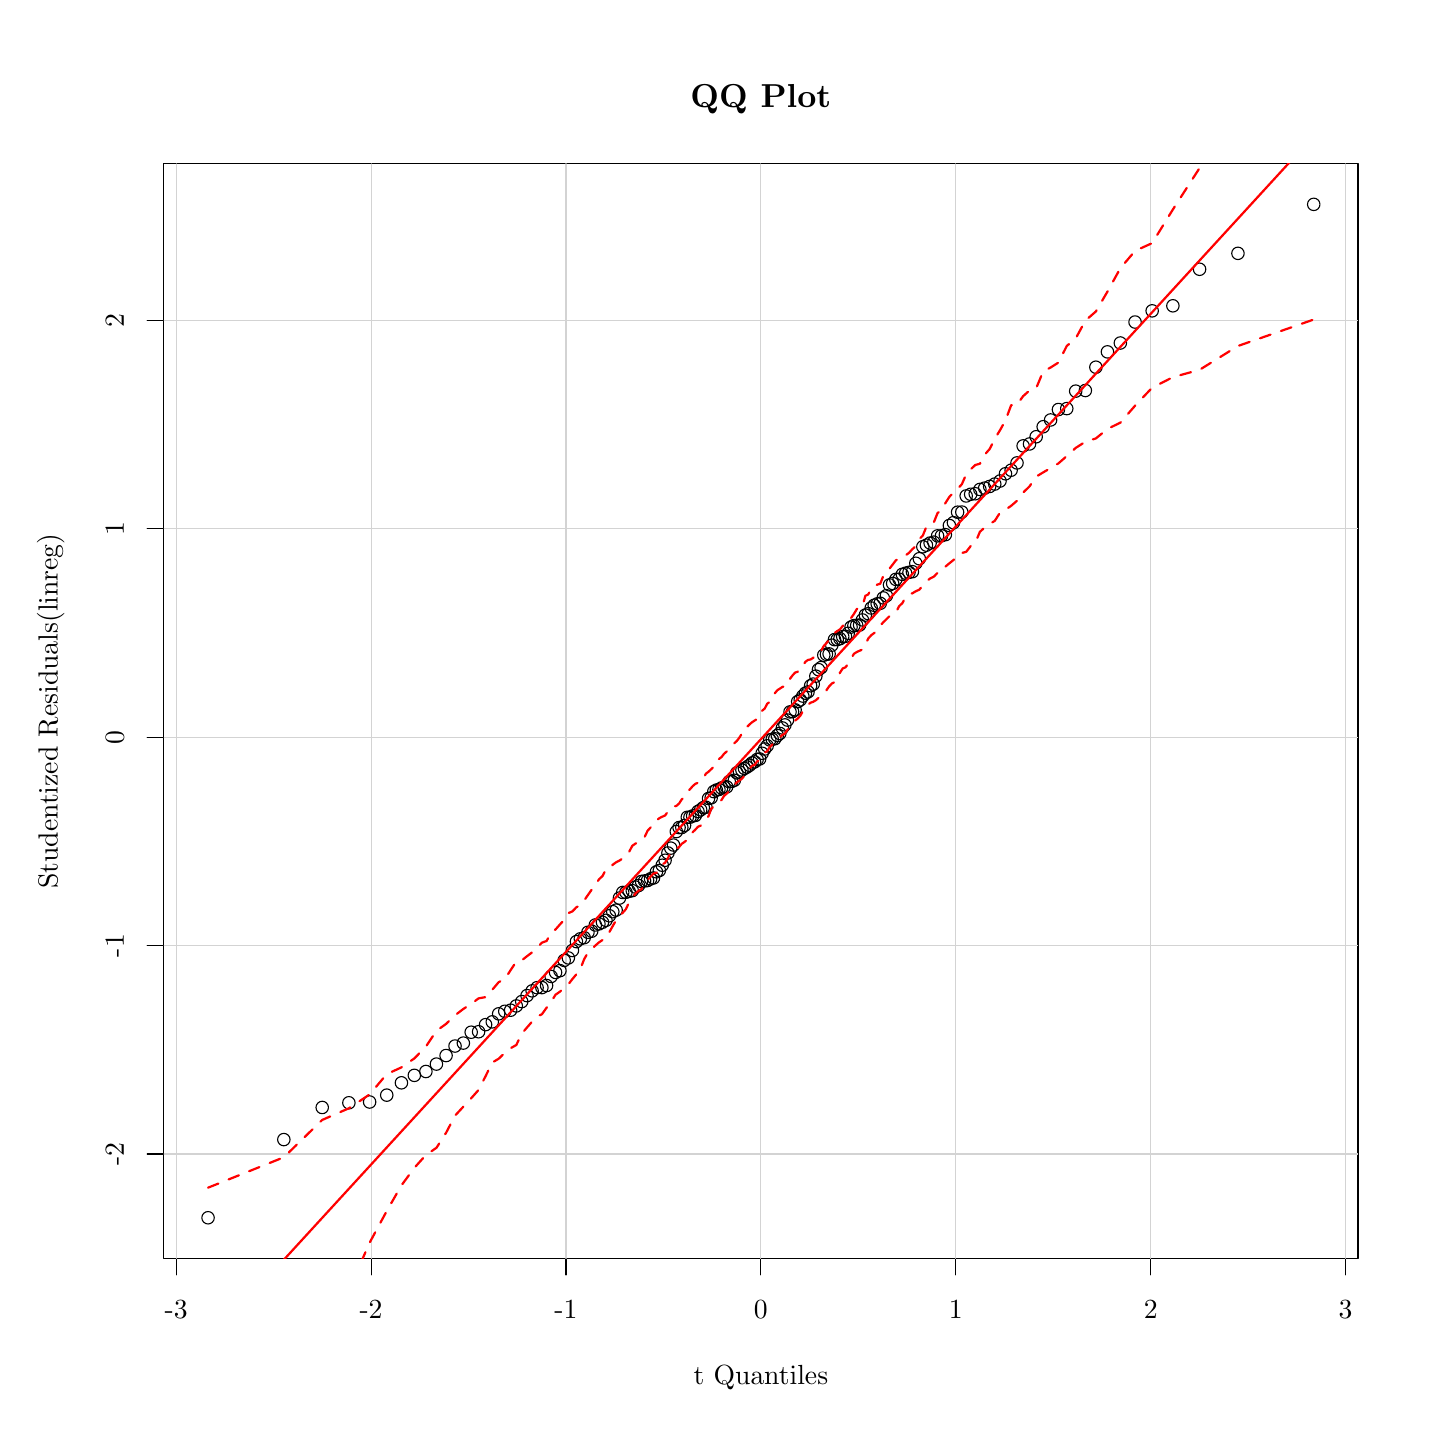
\begin{tikzpicture}[x=1pt,y=1pt]
\definecolor{fillColor}{RGB}{255,255,255}
\path[use as bounding box,fill=fillColor,fill opacity=0.00] (0,0) rectangle (505.89,505.89);
\begin{scope}
\path[clip] (  0.00,  0.00) rectangle (505.89,505.89);
\definecolor{drawColor}{RGB}{0,0,0}

\path[draw=drawColor,line width= 0.4pt,line join=round,line cap=round] ( 53.65, 61.20) -- (476.24, 61.20);

\path[draw=drawColor,line width= 0.4pt,line join=round,line cap=round] ( 53.65, 61.20) -- ( 53.65, 55.20);

\path[draw=drawColor,line width= 0.4pt,line join=round,line cap=round] (124.08, 61.20) -- (124.08, 55.20);

\path[draw=drawColor,line width= 0.4pt,line join=round,line cap=round] (194.51, 61.20) -- (194.51, 55.20);

\path[draw=drawColor,line width= 0.4pt,line join=round,line cap=round] (264.94, 61.20) -- (264.94, 55.20);

\path[draw=drawColor,line width= 0.4pt,line join=round,line cap=round] (335.38, 61.20) -- (335.38, 55.20);

\path[draw=drawColor,line width= 0.4pt,line join=round,line cap=round] (405.81, 61.20) -- (405.81, 55.20);

\path[draw=drawColor,line width= 0.4pt,line join=round,line cap=round] (476.24, 61.20) -- (476.24, 55.20);

\node[text=drawColor,anchor=base,inner sep=0pt, outer sep=0pt, scale=  1.00] at ( 53.65, 39.60) {-3};

\node[text=drawColor,anchor=base,inner sep=0pt, outer sep=0pt, scale=  1.00] at (124.08, 39.60) {-2};

\node[text=drawColor,anchor=base,inner sep=0pt, outer sep=0pt, scale=  1.00] at (194.51, 39.60) {-1};

\node[text=drawColor,anchor=base,inner sep=0pt, outer sep=0pt, scale=  1.00] at (264.94, 39.60) {0};

\node[text=drawColor,anchor=base,inner sep=0pt, outer sep=0pt, scale=  1.00] at (335.38, 39.60) {1};

\node[text=drawColor,anchor=base,inner sep=0pt, outer sep=0pt, scale=  1.00] at (405.81, 39.60) {2};

\node[text=drawColor,anchor=base,inner sep=0pt, outer sep=0pt, scale=  1.00] at (476.24, 39.60) {3};

\path[draw=drawColor,line width= 0.4pt,line join=round,line cap=round] ( 49.20, 98.89) -- ( 49.20,400.13);

\path[draw=drawColor,line width= 0.4pt,line join=round,line cap=round] ( 49.20, 98.89) -- ( 43.20, 98.89);

\path[draw=drawColor,line width= 0.4pt,line join=round,line cap=round] ( 49.20,174.20) -- ( 43.20,174.20);

\path[draw=drawColor,line width= 0.4pt,line join=round,line cap=round] ( 49.20,249.51) -- ( 43.20,249.51);

\path[draw=drawColor,line width= 0.4pt,line join=round,line cap=round] ( 49.20,324.82) -- ( 43.20,324.82);

\path[draw=drawColor,line width= 0.4pt,line join=round,line cap=round] ( 49.20,400.13) -- ( 43.20,400.13);

\node[text=drawColor,rotate= 90.00,anchor=base,inner sep=0pt, outer sep=0pt, scale=  1.00] at ( 34.80, 98.89) {-2};

\node[text=drawColor,rotate= 90.00,anchor=base,inner sep=0pt, outer sep=0pt, scale=  1.00] at ( 34.80,174.20) {-1};

\node[text=drawColor,rotate= 90.00,anchor=base,inner sep=0pt, outer sep=0pt, scale=  1.00] at ( 34.80,249.51) {0};

\node[text=drawColor,rotate= 90.00,anchor=base,inner sep=0pt, outer sep=0pt, scale=  1.00] at ( 34.80,324.82) {1};

\node[text=drawColor,rotate= 90.00,anchor=base,inner sep=0pt, outer sep=0pt, scale=  1.00] at ( 34.80,400.13) {2};

\path[draw=drawColor,line width= 0.4pt,line join=round,line cap=round] ( 49.20, 61.20) --
	(480.69, 61.20) --
	(480.69,456.69) --
	( 49.20,456.69) --
	( 49.20, 61.20);
\end{scope}
\begin{scope}
\path[clip] (  0.00,  0.00) rectangle (505.89,505.89);
\definecolor{drawColor}{RGB}{0,0,0}

\node[text=drawColor,anchor=base,inner sep=0pt, outer sep=0pt, scale=  1.20] at (264.94,477.15) {\bfseries QQ Plot};

\node[text=drawColor,anchor=base,inner sep=0pt, outer sep=0pt, scale=  1.00] at (264.94, 15.60) {t Quantiles};

\node[text=drawColor,rotate= 90.00,anchor=base,inner sep=0pt, outer sep=0pt, scale=  1.00] at ( 10.80,258.94) {Studentized Residuals(linreg)};
\end{scope}
\begin{scope}
\path[clip] ( 49.20, 61.20) rectangle (480.69,456.69);
\definecolor{drawColor}{RGB}{211,211,211}

\path[draw=drawColor,line width= 0.4pt,line join=round,line cap=round] ( 53.65, 61.20) -- ( 53.65,456.69);

\path[draw=drawColor,line width= 0.4pt,line join=round,line cap=round] (124.08, 61.20) -- (124.08,456.69);

\path[draw=drawColor,line width= 0.4pt,line join=round,line cap=round] (194.51, 61.20) -- (194.51,456.69);

\path[draw=drawColor,line width= 0.4pt,line join=round,line cap=round] (264.94, 61.20) -- (264.94,456.69);

\path[draw=drawColor,line width= 0.4pt,line join=round,line cap=round] (335.38, 61.20) -- (335.38,456.69);

\path[draw=drawColor,line width= 0.4pt,line join=round,line cap=round] (405.81, 61.20) -- (405.81,456.69);

\path[draw=drawColor,line width= 0.4pt,line join=round,line cap=round] (476.24, 61.20) -- (476.24,456.69);

\path[draw=drawColor,line width= 0.4pt,line join=round,line cap=round] ( 49.20, 98.89) -- (480.69, 98.89);

\path[draw=drawColor,line width= 0.4pt,line join=round,line cap=round] ( 49.20,174.20) -- (480.69,174.20);

\path[draw=drawColor,line width= 0.4pt,line join=round,line cap=round] ( 49.20,249.51) -- (480.69,249.51);

\path[draw=drawColor,line width= 0.4pt,line join=round,line cap=round] ( 49.20,324.82) -- (480.69,324.82);

\path[draw=drawColor,line width= 0.4pt,line join=round,line cap=round] ( 49.20,400.13) -- (480.69,400.13);
\definecolor{drawColor}{RGB}{0,0,0}

\path[draw=drawColor,line width= 0.4pt,line join=round,line cap=round] ( 65.18, 75.85) circle (  2.25);

\path[draw=drawColor,line width= 0.4pt,line join=round,line cap=round] ( 92.56,104.10) circle (  2.25);

\path[draw=drawColor,line width= 0.4pt,line join=round,line cap=round] (106.43,115.70) circle (  2.25);

\path[draw=drawColor,line width= 0.4pt,line join=round,line cap=round] (116.07,117.40) circle (  2.25);

\path[draw=drawColor,line width= 0.4pt,line join=round,line cap=round] (123.56,117.68) circle (  2.25);

\path[draw=drawColor,line width= 0.4pt,line join=round,line cap=round] (129.75,120.16) circle (  2.25);

\path[draw=drawColor,line width= 0.4pt,line join=round,line cap=round] (135.06,124.61) circle (  2.25);

\path[draw=drawColor,line width= 0.4pt,line join=round,line cap=round] (139.72,127.31) circle (  2.25);

\path[draw=drawColor,line width= 0.4pt,line join=round,line cap=round] (143.90,128.70) circle (  2.25);

\path[draw=drawColor,line width= 0.4pt,line join=round,line cap=round] (147.70,131.38) circle (  2.25);

\path[draw=drawColor,line width= 0.4pt,line join=round,line cap=round] (151.19,134.47) circle (  2.25);

\path[draw=drawColor,line width= 0.4pt,line join=round,line cap=round] (154.42,137.90) circle (  2.25);

\path[draw=drawColor,line width= 0.4pt,line join=round,line cap=round] (157.43,138.97) circle (  2.25);

\path[draw=drawColor,line width= 0.4pt,line join=round,line cap=round] (160.26,142.90) circle (  2.25);

\path[draw=drawColor,line width= 0.4pt,line join=round,line cap=round] (162.94,143.07) circle (  2.25);

\path[draw=drawColor,line width= 0.4pt,line join=round,line cap=round] (165.47,145.64) circle (  2.25);

\path[draw=drawColor,line width= 0.4pt,line join=round,line cap=round] (167.88,146.63) circle (  2.25);

\path[draw=drawColor,line width= 0.4pt,line join=round,line cap=round] (170.19,149.54) circle (  2.25);

\path[draw=drawColor,line width= 0.4pt,line join=round,line cap=round] (172.40,150.46) circle (  2.25);

\path[draw=drawColor,line width= 0.4pt,line join=round,line cap=round] (174.52,150.85) circle (  2.25);

\path[draw=drawColor,line width= 0.4pt,line join=round,line cap=round] (176.56,152.39) circle (  2.25);

\path[draw=drawColor,line width= 0.4pt,line join=round,line cap=round] (178.53,153.96) circle (  2.25);

\path[draw=drawColor,line width= 0.4pt,line join=round,line cap=round] (180.44,156.12) circle (  2.25);

\path[draw=drawColor,line width= 0.4pt,line join=round,line cap=round] (182.28,157.84) circle (  2.25);

\path[draw=drawColor,line width= 0.4pt,line join=round,line cap=round] (184.07,158.99) circle (  2.25);

\path[draw=drawColor,line width= 0.4pt,line join=round,line cap=round] (185.81,159.02) circle (  2.25);

\path[draw=drawColor,line width= 0.4pt,line join=round,line cap=round] (187.50,159.77) circle (  2.25);

\path[draw=drawColor,line width= 0.4pt,line join=round,line cap=round] (189.15,163.04) circle (  2.25);

\path[draw=drawColor,line width= 0.4pt,line join=round,line cap=round] (190.76,164.49) circle (  2.25);

\path[draw=drawColor,line width= 0.4pt,line join=round,line cap=round] (192.33,165.15) circle (  2.25);

\path[draw=drawColor,line width= 0.4pt,line join=round,line cap=round] (193.87,168.85) circle (  2.25);

\path[draw=drawColor,line width= 0.4pt,line join=round,line cap=round] (195.37,169.74) circle (  2.25);

\path[draw=drawColor,line width= 0.4pt,line join=round,line cap=round] (196.84,172.43) circle (  2.25);

\path[draw=drawColor,line width= 0.4pt,line join=round,line cap=round] (198.29,175.64) circle (  2.25);

\path[draw=drawColor,line width= 0.4pt,line join=round,line cap=round] (199.70,176.64) circle (  2.25);

\path[draw=drawColor,line width= 0.4pt,line join=round,line cap=round] (201.09,177.05) circle (  2.25);

\path[draw=drawColor,line width= 0.4pt,line join=round,line cap=round] (202.46,179.01) circle (  2.25);

\path[draw=drawColor,line width= 0.4pt,line join=round,line cap=round] (203.80,179.40) circle (  2.25);

\path[draw=drawColor,line width= 0.4pt,line join=round,line cap=round] (205.12,181.65) circle (  2.25);

\path[draw=drawColor,line width= 0.4pt,line join=round,line cap=round] (206.42,182.04) circle (  2.25);

\path[draw=drawColor,line width= 0.4pt,line join=round,line cap=round] (207.70,182.63) circle (  2.25);

\path[draw=drawColor,line width= 0.4pt,line join=round,line cap=round] (208.96,183.33) circle (  2.25);

\path[draw=drawColor,line width= 0.4pt,line join=round,line cap=round] (210.20,184.97) circle (  2.25);

\path[draw=drawColor,line width= 0.4pt,line join=round,line cap=round] (211.43,186.44) circle (  2.25);

\path[draw=drawColor,line width= 0.4pt,line join=round,line cap=round] (212.64,187.02) circle (  2.25);

\path[draw=drawColor,line width= 0.4pt,line join=round,line cap=round] (213.83,191.36) circle (  2.25);

\path[draw=drawColor,line width= 0.4pt,line join=round,line cap=round] (215.01,193.39) circle (  2.25);

\path[draw=drawColor,line width= 0.4pt,line join=round,line cap=round] (216.18,193.45) circle (  2.25);

\path[draw=drawColor,line width= 0.4pt,line join=round,line cap=round] (217.33,193.83) circle (  2.25);

\path[draw=drawColor,line width= 0.4pt,line join=round,line cap=round] (218.47,194.05) circle (  2.25);

\path[draw=drawColor,line width= 0.4pt,line join=round,line cap=round] (219.60,195.35) circle (  2.25);

\path[draw=drawColor,line width= 0.4pt,line join=round,line cap=round] (220.72,195.90) circle (  2.25);

\path[draw=drawColor,line width= 0.4pt,line join=round,line cap=round] (221.82,197.37) circle (  2.25);

\path[draw=drawColor,line width= 0.4pt,line join=round,line cap=round] (222.92,197.56) circle (  2.25);

\path[draw=drawColor,line width= 0.4pt,line join=round,line cap=round] (224.00,197.72) circle (  2.25);

\path[draw=drawColor,line width= 0.4pt,line join=round,line cap=round] (225.08,198.33) circle (  2.25);

\path[draw=drawColor,line width= 0.4pt,line join=round,line cap=round] (226.14,198.64) circle (  2.25);

\path[draw=drawColor,line width= 0.4pt,line join=round,line cap=round] (227.20,200.86) circle (  2.25);

\path[draw=drawColor,line width= 0.4pt,line join=round,line cap=round] (228.25,201.35) circle (  2.25);

\path[draw=drawColor,line width= 0.4pt,line join=round,line cap=round] (229.29,203.24) circle (  2.25);

\path[draw=drawColor,line width= 0.4pt,line join=round,line cap=round] (230.32,205.03) circle (  2.25);

\path[draw=drawColor,line width= 0.4pt,line join=round,line cap=round] (231.35,207.66) circle (  2.25);

\path[draw=drawColor,line width= 0.4pt,line join=round,line cap=round] (232.37,209.42) circle (  2.25);

\path[draw=drawColor,line width= 0.4pt,line join=round,line cap=round] (233.38,210.53) circle (  2.25);

\path[draw=drawColor,line width= 0.4pt,line join=round,line cap=round] (234.38,215.40) circle (  2.25);

\path[draw=drawColor,line width= 0.4pt,line join=round,line cap=round] (235.38,216.85) circle (  2.25);

\path[draw=drawColor,line width= 0.4pt,line join=round,line cap=round] (236.38,216.88) circle (  2.25);

\path[draw=drawColor,line width= 0.4pt,line join=round,line cap=round] (237.36,217.62) circle (  2.25);

\path[draw=drawColor,line width= 0.4pt,line join=round,line cap=round] (238.35,220.56) circle (  2.25);

\path[draw=drawColor,line width= 0.4pt,line join=round,line cap=round] (239.32,220.59) circle (  2.25);

\path[draw=drawColor,line width= 0.4pt,line join=round,line cap=round] (240.29,221.05) circle (  2.25);

\path[draw=drawColor,line width= 0.4pt,line join=round,line cap=round] (241.26,221.23) circle (  2.25);

\path[draw=drawColor,line width= 0.4pt,line join=round,line cap=round] (242.22,222.65) circle (  2.25);

\path[draw=drawColor,line width= 0.4pt,line join=round,line cap=round] (243.18,223.25) circle (  2.25);

\path[draw=drawColor,line width= 0.4pt,line join=round,line cap=round] (244.14,224.04) circle (  2.25);

\path[draw=drawColor,line width= 0.4pt,line join=round,line cap=round] (245.09,224.18) circle (  2.25);

\path[draw=drawColor,line width= 0.4pt,line join=round,line cap=round] (246.03,227.35) circle (  2.25);

\path[draw=drawColor,line width= 0.4pt,line join=round,line cap=round] (246.98,227.59) circle (  2.25);

\path[draw=drawColor,line width= 0.4pt,line join=round,line cap=round] (247.92,229.83) circle (  2.25);

\path[draw=drawColor,line width= 0.4pt,line join=round,line cap=round] (248.85,230.39) circle (  2.25);

\path[draw=drawColor,line width= 0.4pt,line join=round,line cap=round] (249.79,230.61) circle (  2.25);

\path[draw=drawColor,line width= 0.4pt,line join=round,line cap=round] (250.72,231.15) circle (  2.25);

\path[draw=drawColor,line width= 0.4pt,line join=round,line cap=round] (251.65,231.45) circle (  2.25);

\path[draw=drawColor,line width= 0.4pt,line join=round,line cap=round] (252.58,231.55) circle (  2.25);

\path[draw=drawColor,line width= 0.4pt,line join=round,line cap=round] (253.50,233.47) circle (  2.25);

\path[draw=drawColor,line width= 0.4pt,line join=round,line cap=round] (254.42,233.53) circle (  2.25);

\path[draw=drawColor,line width= 0.4pt,line join=round,line cap=round] (255.34,233.94) circle (  2.25);

\path[draw=drawColor,line width= 0.4pt,line join=round,line cap=round] (256.26,236.62) circle (  2.25);

\path[draw=drawColor,line width= 0.4pt,line join=round,line cap=round] (257.18,236.95) circle (  2.25);

\path[draw=drawColor,line width= 0.4pt,line join=round,line cap=round] (258.10,237.62) circle (  2.25);

\path[draw=drawColor,line width= 0.4pt,line join=round,line cap=round] (259.01,238.22) circle (  2.25);

\path[draw=drawColor,line width= 0.4pt,line join=round,line cap=round] (259.93,238.72) circle (  2.25);

\path[draw=drawColor,line width= 0.4pt,line join=round,line cap=round] (260.84,239.36) circle (  2.25);

\path[draw=drawColor,line width= 0.4pt,line join=round,line cap=round] (261.75,240.18) circle (  2.25);

\path[draw=drawColor,line width= 0.4pt,line join=round,line cap=round] (262.67,240.58) circle (  2.25);

\path[draw=drawColor,line width= 0.4pt,line join=round,line cap=round] (263.58,241.44) circle (  2.25);

\path[draw=drawColor,line width= 0.4pt,line join=round,line cap=round] (264.49,241.64) circle (  2.25);

\path[draw=drawColor,line width= 0.4pt,line join=round,line cap=round] (265.40,243.69) circle (  2.25);

\path[draw=drawColor,line width= 0.4pt,line join=round,line cap=round] (266.31,245.23) circle (  2.25);

\path[draw=drawColor,line width= 0.4pt,line join=round,line cap=round] (267.22,246.38) circle (  2.25);

\path[draw=drawColor,line width= 0.4pt,line join=round,line cap=round] (268.14,248.51) circle (  2.25);

\path[draw=drawColor,line width= 0.4pt,line join=round,line cap=round] (269.05,248.76) circle (  2.25);

\path[draw=drawColor,line width= 0.4pt,line join=round,line cap=round] (269.96,248.94) circle (  2.25);

\path[draw=drawColor,line width= 0.4pt,line join=round,line cap=round] (270.88,250.12) circle (  2.25);

\path[draw=drawColor,line width= 0.4pt,line join=round,line cap=round] (271.79,250.85) circle (  2.25);

\path[draw=drawColor,line width= 0.4pt,line join=round,line cap=round] (272.71,252.84) circle (  2.25);

\path[draw=drawColor,line width= 0.4pt,line join=round,line cap=round] (273.63,253.94) circle (  2.25);

\path[draw=drawColor,line width= 0.4pt,line join=round,line cap=round] (274.55,255.69) circle (  2.25);

\path[draw=drawColor,line width= 0.4pt,line join=round,line cap=round] (275.47,258.64) circle (  2.25);

\path[draw=drawColor,line width= 0.4pt,line join=round,line cap=round] (276.39,258.75) circle (  2.25);

\path[draw=drawColor,line width= 0.4pt,line join=round,line cap=round] (277.31,259.39) circle (  2.25);

\path[draw=drawColor,line width= 0.4pt,line join=round,line cap=round] (278.24,262.33) circle (  2.25);

\path[draw=drawColor,line width= 0.4pt,line join=round,line cap=round] (279.17,262.98) circle (  2.25);

\path[draw=drawColor,line width= 0.4pt,line join=round,line cap=round] (280.10,264.36) circle (  2.25);

\path[draw=drawColor,line width= 0.4pt,line join=round,line cap=round] (281.04,265.41) circle (  2.25);

\path[draw=drawColor,line width= 0.4pt,line join=round,line cap=round] (281.97,265.87) circle (  2.25);

\path[draw=drawColor,line width= 0.4pt,line join=round,line cap=round] (282.91,268.09) circle (  2.25);

\path[draw=drawColor,line width= 0.4pt,line join=round,line cap=round] (283.86,268.69) circle (  2.25);

\path[draw=drawColor,line width= 0.4pt,line join=round,line cap=round] (284.80,271.56) circle (  2.25);

\path[draw=drawColor,line width= 0.4pt,line join=round,line cap=round] (285.75,273.91) circle (  2.25);

\path[draw=drawColor,line width= 0.4pt,line join=round,line cap=round] (286.71,274.65) circle (  2.25);

\path[draw=drawColor,line width= 0.4pt,line join=round,line cap=round] (287.67,279.13) circle (  2.25);

\path[draw=drawColor,line width= 0.4pt,line join=round,line cap=round] (288.63,279.46) circle (  2.25);

\path[draw=drawColor,line width= 0.4pt,line join=round,line cap=round] (289.60,279.60) circle (  2.25);

\path[draw=drawColor,line width= 0.4pt,line join=round,line cap=round] (290.57,282.75) circle (  2.25);

\path[draw=drawColor,line width= 0.4pt,line join=round,line cap=round] (291.54,284.76) circle (  2.25);

\path[draw=drawColor,line width= 0.4pt,line join=round,line cap=round] (292.53,284.79) circle (  2.25);

\path[draw=drawColor,line width= 0.4pt,line join=round,line cap=round] (293.51,285.09) circle (  2.25);

\path[draw=drawColor,line width= 0.4pt,line join=round,line cap=round] (294.51,285.86) circle (  2.25);

\path[draw=drawColor,line width= 0.4pt,line join=round,line cap=round] (295.51,285.95) circle (  2.25);

\path[draw=drawColor,line width= 0.4pt,line join=round,line cap=round] (296.51,287.05) circle (  2.25);

\path[draw=drawColor,line width= 0.4pt,line join=round,line cap=round] (297.52,289.29) circle (  2.25);

\path[draw=drawColor,line width= 0.4pt,line join=round,line cap=round] (298.54,289.81) circle (  2.25);

\path[draw=drawColor,line width= 0.4pt,line join=round,line cap=round] (299.57,289.92) circle (  2.25);

\path[draw=drawColor,line width= 0.4pt,line join=round,line cap=round] (300.60,290.04) circle (  2.25);

\path[draw=drawColor,line width= 0.4pt,line join=round,line cap=round] (301.64,291.87) circle (  2.25);

\path[draw=drawColor,line width= 0.4pt,line join=round,line cap=round] (302.69,293.62) circle (  2.25);

\path[draw=drawColor,line width= 0.4pt,line join=round,line cap=round] (303.75,294.13) circle (  2.25);

\path[draw=drawColor,line width= 0.4pt,line join=round,line cap=round] (304.81,296.19) circle (  2.25);

\path[draw=drawColor,line width= 0.4pt,line join=round,line cap=round] (305.89,297.17) circle (  2.25);

\path[draw=drawColor,line width= 0.4pt,line join=round,line cap=round] (306.97,297.67) circle (  2.25);

\path[draw=drawColor,line width= 0.4pt,line join=round,line cap=round] (308.07,297.89) circle (  2.25);

\path[draw=drawColor,line width= 0.4pt,line join=round,line cap=round] (309.17,299.82) circle (  2.25);

\path[draw=drawColor,line width= 0.4pt,line join=round,line cap=round] (310.29,300.62) circle (  2.25);

\path[draw=drawColor,line width= 0.4pt,line join=round,line cap=round] (311.42,304.53) circle (  2.25);

\path[draw=drawColor,line width= 0.4pt,line join=round,line cap=round] (312.56,305.05) circle (  2.25);

\path[draw=drawColor,line width= 0.4pt,line join=round,line cap=round] (313.71,306.54) circle (  2.25);

\path[draw=drawColor,line width= 0.4pt,line join=round,line cap=round] (314.88,306.60) circle (  2.25);

\path[draw=drawColor,line width= 0.4pt,line join=round,line cap=round] (316.06,308.35) circle (  2.25);

\path[draw=drawColor,line width= 0.4pt,line join=round,line cap=round] (317.25,308.76) circle (  2.25);

\path[draw=drawColor,line width= 0.4pt,line join=round,line cap=round] (318.46,309.07) circle (  2.25);

\path[draw=drawColor,line width= 0.4pt,line join=round,line cap=round] (319.69,309.30) circle (  2.25);

\path[draw=drawColor,line width= 0.4pt,line join=round,line cap=round] (320.93,312.35) circle (  2.25);

\path[draw=drawColor,line width= 0.4pt,line join=round,line cap=round] (322.19,313.99) circle (  2.25);

\path[draw=drawColor,line width= 0.4pt,line join=round,line cap=round] (323.47,318.32) circle (  2.25);

\path[draw=drawColor,line width= 0.4pt,line join=round,line cap=round] (324.77,318.89) circle (  2.25);

\path[draw=drawColor,line width= 0.4pt,line join=round,line cap=round] (326.09,319.65) circle (  2.25);

\path[draw=drawColor,line width= 0.4pt,line join=round,line cap=round] (327.43,319.97) circle (  2.25);

\path[draw=drawColor,line width= 0.4pt,line join=round,line cap=round] (328.80,322.25) circle (  2.25);

\path[draw=drawColor,line width= 0.4pt,line join=round,line cap=round] (330.19,322.27) circle (  2.25);

\path[draw=drawColor,line width= 0.4pt,line join=round,line cap=round] (331.60,322.68) circle (  2.25);

\path[draw=drawColor,line width= 0.4pt,line join=round,line cap=round] (333.05,326.00) circle (  2.25);

\path[draw=drawColor,line width= 0.4pt,line join=round,line cap=round] (334.52,327.01) circle (  2.25);

\path[draw=drawColor,line width= 0.4pt,line join=round,line cap=round] (336.02,330.80) circle (  2.25);

\path[draw=drawColor,line width= 0.4pt,line join=round,line cap=round] (337.56,330.85) circle (  2.25);

\path[draw=drawColor,line width= 0.4pt,line join=round,line cap=round] (339.13,336.67) circle (  2.25);

\path[draw=drawColor,line width= 0.4pt,line join=round,line cap=round] (340.74,337.28) circle (  2.25);

\path[draw=drawColor,line width= 0.4pt,line join=round,line cap=round] (342.39,337.47) circle (  2.25);

\path[draw=drawColor,line width= 0.4pt,line join=round,line cap=round] (344.08,339.02) circle (  2.25);

\path[draw=drawColor,line width= 0.4pt,line join=round,line cap=round] (345.82,339.51) circle (  2.25);

\path[draw=drawColor,line width= 0.4pt,line join=round,line cap=round] (347.61,340.10) circle (  2.25);

\path[draw=drawColor,line width= 0.4pt,line join=round,line cap=round] (349.45,340.97) circle (  2.25);

\path[draw=drawColor,line width= 0.4pt,line join=round,line cap=round] (351.36,342.07) circle (  2.25);

\path[draw=drawColor,line width= 0.4pt,line join=round,line cap=round] (353.33,344.69) circle (  2.25);

\path[draw=drawColor,line width= 0.4pt,line join=round,line cap=round] (355.37,345.98) circle (  2.25);

\path[draw=drawColor,line width= 0.4pt,line join=round,line cap=round] (357.49,348.61) circle (  2.25);

\path[draw=drawColor,line width= 0.4pt,line join=round,line cap=round] (359.70,354.76) circle (  2.25);

\path[draw=drawColor,line width= 0.4pt,line join=round,line cap=round] (362.01,355.46) circle (  2.25);

\path[draw=drawColor,line width= 0.4pt,line join=round,line cap=round] (364.42,358.07) circle (  2.25);

\path[draw=drawColor,line width= 0.4pt,line join=round,line cap=round] (366.95,361.68) circle (  2.25);

\path[draw=drawColor,line width= 0.4pt,line join=round,line cap=round] (369.63,364.13) circle (  2.25);

\path[draw=drawColor,line width= 0.4pt,line join=round,line cap=round] (372.46,367.90) circle (  2.25);

\path[draw=drawColor,line width= 0.4pt,line join=round,line cap=round] (375.47,368.24) circle (  2.25);

\path[draw=drawColor,line width= 0.4pt,line join=round,line cap=round] (378.70,374.55) circle (  2.25);

\path[draw=drawColor,line width= 0.4pt,line join=round,line cap=round] (382.19,374.78) circle (  2.25);

\path[draw=drawColor,line width= 0.4pt,line join=round,line cap=round] (385.99,383.20) circle (  2.25);

\path[draw=drawColor,line width= 0.4pt,line join=round,line cap=round] (390.17,388.74) circle (  2.25);

\path[draw=drawColor,line width= 0.4pt,line join=round,line cap=round] (394.83,391.94) circle (  2.25);

\path[draw=drawColor,line width= 0.4pt,line join=round,line cap=round] (400.14,399.52) circle (  2.25);

\path[draw=drawColor,line width= 0.4pt,line join=round,line cap=round] (406.33,403.56) circle (  2.25);

\path[draw=drawColor,line width= 0.4pt,line join=round,line cap=round] (413.82,405.38) circle (  2.25);

\path[draw=drawColor,line width= 0.4pt,line join=round,line cap=round] (423.46,418.59) circle (  2.25);

\path[draw=drawColor,line width= 0.4pt,line join=round,line cap=round] (437.33,424.34) circle (  2.25);

\path[draw=drawColor,line width= 0.4pt,line join=round,line cap=round] (464.71,442.04) circle (  2.25);
\definecolor{drawColor}{RGB}{255,0,0}

\path[draw=drawColor,line width= 0.8pt,dash pattern=on 4pt off 4pt ,line join=round,line cap=round] ( 65.18, 86.72) --
	( 92.56, 97.70) --
	(106.43,111.20) --
	(116.07,115.41) --
	(123.56,120.42) --
	(129.75,127.75) --
	(135.06,130.19) --
	(139.72,133.42) --
	(143.90,137.71) --
	(147.70,143.39) --
	(151.19,145.90) --
	(154.42,149.01) --
	(157.43,151.30) --
	(160.26,153.13) --
	(162.94,155.13) --
	(165.47,155.59) --
	(167.88,158.23) --
	(170.19,160.98) --
	(172.40,162.10) --
	(174.52,165.33) --
	(176.56,168.40) --
	(178.53,168.86) --
	(180.44,170.37) --
	(182.28,171.76) --
	(184.07,173.43) --
	(185.81,175.26) --
	(187.50,175.86) --
	(189.15,178.89) --
	(190.76,180.05) --
	(192.33,181.84) --
	(193.87,183.50) --
	(195.37,185.93) --
	(196.84,186.56) --
	(198.29,188.07) --
	(199.70,188.75) --
	(201.09,190.50) --
	(202.46,192.50) --
	(203.80,194.40) --
	(205.12,195.92) --
	(206.42,198.13) --
	(207.70,199.31) --
	(208.96,201.71) --
	(210.20,201.95) --
	(211.43,203.44) --
	(212.64,204.30) --
	(213.83,204.90) --
	(215.01,205.73) --
	(216.18,207.16) --
	(217.33,208.06) --
	(218.47,210.25) --
	(219.60,211.04) --
	(220.72,211.63) --
	(221.82,212.57) --
	(222.92,213.40) --
	(224.00,215.69) --
	(225.08,216.87) --
	(226.14,217.66) --
	(227.20,219.41) --
	(228.25,220.23) --
	(229.29,220.76) --
	(230.32,221.21) --
	(231.35,222.60) --
	(232.37,223.26) --
	(233.38,224.48) --
	(234.38,224.65) --
	(235.38,225.52) --
	(236.38,227.08) --
	(237.36,227.89) --
	(238.35,229.91) --
	(239.32,230.68) --
	(240.29,231.81) --
	(241.26,232.64) --
	(242.22,233.05) --
	(243.18,233.45) --
	(244.14,234.66) --
	(245.09,236.32) --
	(246.03,237.03) --
	(246.98,237.91) --
	(247.92,238.87) --
	(248.85,241.12) --
	(249.79,241.61) --
	(250.72,242.32) --
	(251.65,243.53) --
	(252.58,244.33) --
	(253.50,245.06) --
	(254.42,246.21) --
	(255.34,247.30) --
	(256.26,248.17) --
	(257.18,249.34) --
	(258.10,250.84) --
	(259.01,251.13) --
	(259.93,253.21) --
	(260.84,254.11) --
	(261.75,254.91) --
	(262.67,255.50) --
	(263.58,256.08) --
	(264.49,258.44) --
	(265.40,259.08) --
	(266.31,259.82) --
	(267.22,261.60) --
	(268.14,262.22) --
	(269.05,264.27) --
	(269.96,265.35) --
	(270.88,266.46) --
	(271.79,267.05) --
	(272.71,267.64) --
	(273.63,268.03) --
	(274.55,270.26) --
	(275.47,270.63) --
	(276.39,271.85) --
	(277.31,272.85) --
	(278.24,273.16) --
	(279.17,275.02) --
	(280.10,275.40) --
	(281.04,276.75) --
	(281.97,277.42) --
	(282.91,277.60) --
	(283.86,278.19) --
	(284.80,279.04) --
	(285.75,280.19) --
	(286.71,280.76) --
	(287.67,282.45) --
	(288.63,283.49) --
	(289.60,284.73) --
	(290.57,286.01) --
	(291.54,287.15) --
	(292.53,287.85) --
	(293.51,288.45) --
	(294.51,289.69) --
	(295.51,290.42) --
	(296.51,291.93) --
	(297.52,292.56) --
	(298.54,294.00) --
	(299.57,295.75) --
	(300.60,296.59) --
	(301.64,296.77) --
	(302.69,300.59) --
	(303.75,301.10) --
	(304.81,303.17) --
	(305.89,303.80) --
	(306.97,304.62) --
	(308.07,304.95) --
	(309.17,307.78) --
	(310.29,309.10) --
	(311.42,310.41) --
	(312.56,311.89) --
	(313.71,313.40) --
	(314.88,314.16) --
	(316.06,314.56) --
	(317.25,315.23) --
	(318.46,316.11) --
	(319.69,317.45) --
	(320.93,318.58) --
	(322.19,321.04) --
	(323.47,322.39) --
	(324.77,325.62) --
	(326.09,326.71) --
	(327.43,327.11) --
	(328.80,330.54) --
	(330.19,331.38) --
	(331.60,334.07) --
	(333.05,336.35) --
	(334.52,337.92) --
	(336.02,339.22) --
	(337.56,340.91) --
	(339.13,344.48) --
	(340.74,346.25) --
	(342.39,347.85) --
	(344.08,348.32) --
	(345.82,351.59) --
	(347.61,353.64) --
	(349.45,357.28) --
	(351.36,360.45) --
	(353.33,363.96) --
	(355.37,369.46) --
	(357.49,369.68) --
	(359.70,372.73) --
	(362.01,374.79) --
	(364.42,375.62) --
	(366.95,381.66) --
	(369.63,383.08) --
	(372.46,384.87) --
	(375.47,390.87) --
	(378.70,393.58) --
	(382.19,400.03) --
	(385.99,403.33) --
	(390.17,410.50) --
	(394.83,418.96) --
	(400.14,425.21) --
	(406.33,428.03) --
	(413.82,440.19) --
	(423.46,455.16) --
	(437.33,471.69) --
	(460.70,505.89);

\path[draw=drawColor,line width= 0.8pt,dash pattern=on 4pt off 4pt ,line join=round,line cap=round] ( 83.75,  0.00) --
	( 92.56, 17.00) --
	(106.43, 44.88) --
	(116.07, 49.72) --
	(123.56, 66.84) --
	(129.75, 78.29) --
	(135.06, 87.55) --
	(139.72, 93.88) --
	(143.90, 98.54) --
	(147.70,101.11) --
	(151.19,106.55) --
	(154.42,112.75) --
	(157.43,115.99) --
	(160.26,119.03) --
	(162.94,122.05) --
	(165.47,127.04) --
	(167.88,131.94) --
	(170.19,133.31) --
	(172.40,135.43) --
	(174.52,137.12) --
	(176.56,138.28) --
	(178.53,142.38) --
	(180.44,144.62) --
	(182.28,146.74) --
	(184.07,148.58) --
	(185.81,149.38) --
	(187.50,151.74) --
	(189.15,153.90) --
	(190.76,156.47) --
	(192.33,157.54) --
	(193.87,159.01) --
	(195.37,160.18) --
	(196.84,162.11) --
	(198.29,163.85) --
	(199.70,165.78) --
	(201.09,169.29) --
	(202.46,171.70) --
	(203.80,173.00) --
	(205.12,174.20) --
	(206.42,175.34) --
	(207.70,176.21) --
	(208.96,177.05) --
	(210.20,179.10) --
	(211.43,181.29) --
	(212.64,183.41) --
	(213.83,184.68) --
	(215.01,186.04) --
	(216.18,187.38) --
	(217.33,189.86) --
	(218.47,191.20) --
	(219.60,193.05) --
	(220.72,193.96) --
	(221.82,194.60) --
	(222.92,196.39) --
	(224.00,197.98) --
	(225.08,199.08) --
	(226.14,200.25) --
	(227.20,200.46) --
	(228.25,201.58) --
	(229.29,203.56) --
	(230.32,204.11) --
	(231.35,205.78) --
	(232.37,207.85) --
	(233.38,208.75) --
	(234.38,209.17) --
	(235.38,209.82) --
	(236.38,211.01) --
	(237.36,211.67) --
	(238.35,212.44) --
	(239.32,214.47) --
	(240.29,215.15) --
	(241.26,216.11) --
	(242.22,217.14) --
	(243.18,217.56) --
	(244.14,218.49) --
	(245.09,219.99) --
	(246.03,220.94) --
	(246.98,223.67) --
	(247.92,224.39) --
	(248.85,224.70) --
	(249.79,226.02) --
	(250.72,226.82) --
	(251.65,228.31) --
	(252.58,229.09) --
	(253.50,230.04) --
	(254.42,230.80) --
	(255.34,232.22) --
	(256.26,233.21) --
	(257.18,233.81) --
	(258.10,234.52) --
	(259.01,235.60) --
	(259.93,236.88) --
	(260.84,238.00) --
	(261.75,239.20) --
	(262.67,239.45) --
	(263.58,240.77) --
	(264.49,241.19) --
	(265.40,242.49) --
	(266.31,243.92) --
	(267.22,244.43) --
	(268.14,245.95) --
	(269.05,246.83) --
	(269.96,248.08) --
	(270.88,248.68) --
	(271.79,249.41) --
	(272.71,250.33) --
	(273.63,250.83) --
	(274.55,252.21) --
	(275.47,253.27) --
	(276.39,254.42) --
	(277.31,255.50) --
	(278.24,256.23) --
	(279.17,257.22) --
	(280.10,258.85) --
	(281.04,260.01) --
	(281.97,261.24) --
	(282.91,261.97) --
	(283.86,262.30) --
	(284.80,262.85) --
	(285.75,263.70) --
	(286.71,264.36) --
	(287.67,265.15) --
	(288.63,266.46) --
	(289.60,267.87) --
	(290.57,268.87) --
	(291.54,269.40) --
	(292.53,270.59) --
	(293.51,272.79) --
	(294.51,274.34) --
	(295.51,274.75) --
	(296.51,276.04) --
	(297.52,277.77) --
	(298.54,279.61) --
	(299.57,280.27) --
	(300.60,280.74) --
	(301.64,281.19) --
	(302.69,282.93) --
	(303.75,285.18) --
	(304.81,286.33) --
	(305.89,287.15) --
	(306.97,287.97) --
	(308.07,289.79) --
	(309.17,291.03) --
	(310.29,292.13) --
	(311.42,293.26) --
	(312.56,293.66) --
	(313.71,294.57) --
	(314.88,296.83) --
	(316.06,297.93) --
	(317.25,300.07) --
	(318.46,301.07) --
	(319.69,301.50) --
	(320.93,302.25) --
	(322.19,302.80) --
	(323.47,304.34) --
	(324.77,305.83) --
	(326.09,306.86) --
	(327.43,307.52) --
	(328.80,308.90) --
	(330.19,310.68) --
	(331.60,311.13) --
	(333.05,312.33) --
	(334.52,313.51) --
	(336.02,315.32) --
	(337.56,316.06) --
	(339.13,316.48) --
	(340.74,318.54) --
	(342.39,319.69) --
	(344.08,323.70) --
	(345.82,325.29) --
	(347.61,326.55) --
	(349.45,327.66) --
	(351.36,330.66) --
	(353.33,331.70) --
	(355.37,333.11) --
	(357.49,334.93) --
	(359.70,337.87) --
	(362.01,340.14) --
	(364.42,343.65) --
	(366.95,345.19) --
	(369.63,346.75) --
	(372.46,348.44) --
	(375.47,351.07) --
	(378.70,354.03) --
	(382.19,356.26) --
	(385.99,357.46) --
	(390.17,360.88) --
	(394.83,363.16) --
	(400.14,369.27) --
	(406.33,375.80) --
	(413.82,379.60) --
	(423.46,382.25) --
	(437.33,390.86) --
	(464.71,400.42);

\path[draw=drawColor,line width= 0.8pt,line join=round,line cap=round] ( 49.20, 13.36) -- (480.69,484.20);
\end{scope}
\end{tikzpicture}

	\caption{QQ-Plot}
	\label{fig:qq_plot}
\end{figure}

The bottom tail of the QQ-Plot seems to deviate from the linear line, which is a sign of the error's non-normality. This may mean that the error does not follow a normal model, or that the model is actually non-linear.

\begin{figure}[!hb]
	\centering
	\includegraphics{Figures/fitted_value_plots}
	\caption{}
	\label{fig:fitted_value_plots}
\end{figure}

We can also analyze the Residuals-Fitted plot and the Scale-Location plot to get a better understanding on the model. To do, we can simply apply the function \texttt{plot} on the linear model (figure \ref{fig:fitted_value_plots}).

It turns out that both plots show non-normal scatters of the residuals. In particular, the points displayed in the Residuals-Fitted plot seem to follow a fan shape. This is a sign of a non-constant variance, also called heteroscedasticity.

\section{Measures to Compare Models}
Before building any model, we have to properly define the measures we will later use to compare them. 

\subsection{Some Measures}
A first way to assess the performance of a model is to compute the Mean Squared Error (MSE). We can also use adjusted $R^2$ score.

\subsection{Data Split}
These measures should not be applied on a set whose data was also used to train the model. Indeed, this would include a biais that might distort our conclusions. To cope with this problem, we have to split the dataset into two disjointed sets : 
\begin{itemize}
	\item Training Set : About 75\% of the dataset dedicated to the building the model;
	\item Test Set : The remaining 25\% only used at the end to provide some kind of objective measure of the model performance.
\end{itemize} 

Once it is done, we can finally dive in the model building.

\section{K-nearest neighbors (KNN)}
\subsection{Idea}
We start our analysis with a very simple model called the KNN.
Given an positive integer k and a test observation x0. The KNN model first identifies the k closest points to x0 from the training data. Then estimates \\ 

The KNN model in R is done by calling the function reg of the package knn. As we will see in the following sections, For most prediction algorithms, we first have to build the prediction model on the training data, and then use the model to test our predictions. However, the KNN function does both in a single step.\\ 
In order to find the best k we set a maximum number of neighbors to be considered (in our model it is 20), then we calculate the MSE for each k which is the mean of the squared difference between the real value of Time and the predicted one. All the steps are detailed in the code below.\\

\begin{lstlisting}
library(FNN)
library(tikzDevice)
k_max = 120;
MSE = rep(0,k_max)

for( k in 1:k_max)
{
reg = knn.reg(train=cancer.train.x, test=cancer.test.x, y=cancer.train.y, k=k)
MSE[k] = mean((cancer.test.y - reg$pred)^2)
}

best_k_test = which.min(MSE)
best_k_mse = MSE[best_k_test]
sprintf("Best knn1 = %d and the best MSE1 = %f", best_k_test, best_k_mse)

tikz('Figures/knn.tex',width=5, height=5)

plot(1:k_max, MSE, xlab='k', ylab='MSE', main='MSE against k neighbours')
points(x = best_k_test, y = best_k_mse, col = "red", pch = 16)
abline(h = best_k_mse, col='red')
abline(v = best_k_test, col='red')
dev.off()
\end{lstlisting}

The graph below shows the MSE plotted against the values of k in a range from 1 to 20. We can notice that a minimum is reached between 10 and 20. We use the function which.min that returns the index of the minimum value.\\
	
\begin{figure}[!hb]
	\centering
	% Created by tikzDevice version 0.10.1 on 2016-11-04 23:52:30
% !TEX encoding = UTF-8 Unicode
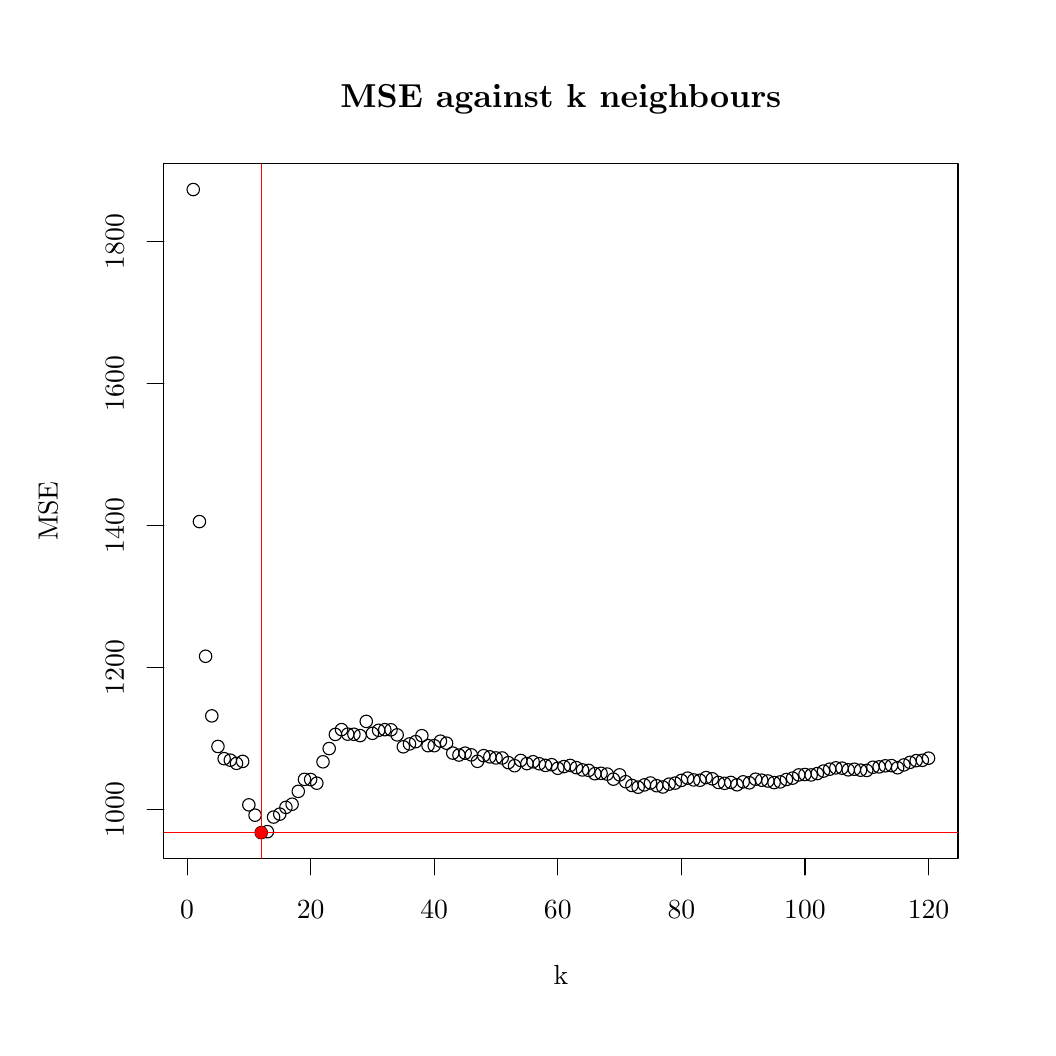
\begin{tikzpicture}[x=1pt,y=1pt]
\definecolor{fillColor}{RGB}{255,255,255}
\path[use as bounding box,fill=fillColor,fill opacity=0.00] (0,0) rectangle (361.35,361.35);
\begin{scope}
\path[clip] ( 49.20, 61.20) rectangle (336.15,312.15);
\definecolor{drawColor}{RGB}{0,0,0}

\path[draw=drawColor,line width= 0.4pt,line join=round,line cap=round] ( 59.83,302.86) circle (  2.25);

\path[draw=drawColor,line width= 0.4pt,line join=round,line cap=round] ( 62.06,182.87) circle (  2.25);

\path[draw=drawColor,line width= 0.4pt,line join=round,line cap=round] ( 64.29,134.21) circle (  2.25);

\path[draw=drawColor,line width= 0.4pt,line join=round,line cap=round] ( 66.53,112.66) circle (  2.25);

\path[draw=drawColor,line width= 0.4pt,line join=round,line cap=round] ( 68.76,101.61) circle (  2.25);

\path[draw=drawColor,line width= 0.4pt,line join=round,line cap=round] ( 70.99, 97.20) circle (  2.25);

\path[draw=drawColor,line width= 0.4pt,line join=round,line cap=round] ( 73.22, 96.66) circle (  2.25);

\path[draw=drawColor,line width= 0.4pt,line join=round,line cap=round] ( 75.46, 95.51) circle (  2.25);

\path[draw=drawColor,line width= 0.4pt,line join=round,line cap=round] ( 77.69, 96.22) circle (  2.25);

\path[draw=drawColor,line width= 0.4pt,line join=round,line cap=round] ( 79.92, 80.51) circle (  2.25);

\path[draw=drawColor,line width= 0.4pt,line join=round,line cap=round] ( 82.16, 76.78) circle (  2.25);

\path[draw=drawColor,line width= 0.4pt,line join=round,line cap=round] ( 84.39, 70.49) circle (  2.25);

\path[draw=drawColor,line width= 0.4pt,line join=round,line cap=round] ( 86.62, 70.83) circle (  2.25);

\path[draw=drawColor,line width= 0.4pt,line join=round,line cap=round] ( 88.85, 76.10) circle (  2.25);

\path[draw=drawColor,line width= 0.4pt,line join=round,line cap=round] ( 91.09, 77.16) circle (  2.25);

\path[draw=drawColor,line width= 0.4pt,line join=round,line cap=round] ( 93.32, 79.60) circle (  2.25);

\path[draw=drawColor,line width= 0.4pt,line join=round,line cap=round] ( 95.55, 80.74) circle (  2.25);

\path[draw=drawColor,line width= 0.4pt,line join=round,line cap=round] ( 97.78, 85.39) circle (  2.25);

\path[draw=drawColor,line width= 0.4pt,line join=round,line cap=round] (100.02, 89.73) circle (  2.25);

\path[draw=drawColor,line width= 0.4pt,line join=round,line cap=round] (102.25, 89.67) circle (  2.25);

\path[draw=drawColor,line width= 0.4pt,line join=round,line cap=round] (104.48, 88.34) circle (  2.25);

\path[draw=drawColor,line width= 0.4pt,line join=round,line cap=round] (106.72, 96.07) circle (  2.25);

\path[draw=drawColor,line width= 0.4pt,line join=round,line cap=round] (108.95,100.86) circle (  2.25);

\path[draw=drawColor,line width= 0.4pt,line join=round,line cap=round] (111.18,105.97) circle (  2.25);

\path[draw=drawColor,line width= 0.4pt,line join=round,line cap=round] (113.41,107.71) circle (  2.25);

\path[draw=drawColor,line width= 0.4pt,line join=round,line cap=round] (115.65,106.06) circle (  2.25);

\path[draw=drawColor,line width= 0.4pt,line join=round,line cap=round] (117.88,106.02) circle (  2.25);

\path[draw=drawColor,line width= 0.4pt,line join=round,line cap=round] (120.11,105.55) circle (  2.25);

\path[draw=drawColor,line width= 0.4pt,line join=round,line cap=round] (122.34,110.67) circle (  2.25);

\path[draw=drawColor,line width= 0.4pt,line join=round,line cap=round] (124.58,106.36) circle (  2.25);

\path[draw=drawColor,line width= 0.4pt,line join=round,line cap=round] (126.81,107.45) circle (  2.25);

\path[draw=drawColor,line width= 0.4pt,line join=round,line cap=round] (129.04,107.68) circle (  2.25);

\path[draw=drawColor,line width= 0.4pt,line join=round,line cap=round] (131.28,107.63) circle (  2.25);

\path[draw=drawColor,line width= 0.4pt,line join=round,line cap=round] (133.51,105.80) circle (  2.25);

\path[draw=drawColor,line width= 0.4pt,line join=round,line cap=round] (135.74,101.49) circle (  2.25);

\path[draw=drawColor,line width= 0.4pt,line join=round,line cap=round] (137.97,102.52) circle (  2.25);

\path[draw=drawColor,line width= 0.4pt,line join=round,line cap=round] (140.21,103.35) circle (  2.25);

\path[draw=drawColor,line width= 0.4pt,line join=round,line cap=round] (142.44,105.51) circle (  2.25);

\path[draw=drawColor,line width= 0.4pt,line join=round,line cap=round] (144.67,101.90) circle (  2.25);

\path[draw=drawColor,line width= 0.4pt,line join=round,line cap=round] (146.90,101.89) circle (  2.25);

\path[draw=drawColor,line width= 0.4pt,line join=round,line cap=round] (149.14,103.53) circle (  2.25);

\path[draw=drawColor,line width= 0.4pt,line join=round,line cap=round] (151.37,102.80) circle (  2.25);

\path[draw=drawColor,line width= 0.4pt,line join=round,line cap=round] (153.60, 99.22) circle (  2.25);

\path[draw=drawColor,line width= 0.4pt,line join=round,line cap=round] (155.84, 98.52) circle (  2.25);

\path[draw=drawColor,line width= 0.4pt,line join=round,line cap=round] (158.07, 99.20) circle (  2.25);

\path[draw=drawColor,line width= 0.4pt,line join=round,line cap=round] (160.30, 98.58) circle (  2.25);

\path[draw=drawColor,line width= 0.4pt,line join=round,line cap=round] (162.53, 96.25) circle (  2.25);

\path[draw=drawColor,line width= 0.4pt,line join=round,line cap=round] (164.77, 98.28) circle (  2.25);

\path[draw=drawColor,line width= 0.4pt,line join=round,line cap=round] (167.00, 97.86) circle (  2.25);

\path[draw=drawColor,line width= 0.4pt,line join=round,line cap=round] (169.23, 97.46) circle (  2.25);

\path[draw=drawColor,line width= 0.4pt,line join=round,line cap=round] (171.46, 97.45) circle (  2.25);

\path[draw=drawColor,line width= 0.4pt,line join=round,line cap=round] (173.70, 95.77) circle (  2.25);

\path[draw=drawColor,line width= 0.4pt,line join=round,line cap=round] (175.93, 94.66) circle (  2.25);

\path[draw=drawColor,line width= 0.4pt,line join=round,line cap=round] (178.16, 96.56) circle (  2.25);

\path[draw=drawColor,line width= 0.4pt,line join=round,line cap=round] (180.40, 95.42) circle (  2.25);

\path[draw=drawColor,line width= 0.4pt,line join=round,line cap=round] (182.63, 96.09) circle (  2.25);

\path[draw=drawColor,line width= 0.4pt,line join=round,line cap=round] (184.86, 95.37) circle (  2.25);

\path[draw=drawColor,line width= 0.4pt,line join=round,line cap=round] (187.09, 94.77) circle (  2.25);

\path[draw=drawColor,line width= 0.4pt,line join=round,line cap=round] (189.33, 95.02) circle (  2.25);

\path[draw=drawColor,line width= 0.4pt,line join=round,line cap=round] (191.56, 93.74) circle (  2.25);

\path[draw=drawColor,line width= 0.4pt,line join=round,line cap=round] (193.79, 94.35) circle (  2.25);

\path[draw=drawColor,line width= 0.4pt,line join=round,line cap=round] (196.02, 94.76) circle (  2.25);

\path[draw=drawColor,line width= 0.4pt,line join=round,line cap=round] (198.26, 93.96) circle (  2.25);

\path[draw=drawColor,line width= 0.4pt,line join=round,line cap=round] (200.49, 93.13) circle (  2.25);

\path[draw=drawColor,line width= 0.4pt,line join=round,line cap=round] (202.72, 92.97) circle (  2.25);

\path[draw=drawColor,line width= 0.4pt,line join=round,line cap=round] (204.95, 91.77) circle (  2.25);

\path[draw=drawColor,line width= 0.4pt,line join=round,line cap=round] (207.19, 91.91) circle (  2.25);

\path[draw=drawColor,line width= 0.4pt,line join=round,line cap=round] (209.42, 91.63) circle (  2.25);

\path[draw=drawColor,line width= 0.4pt,line join=round,line cap=round] (211.65, 89.80) circle (  2.25);

\path[draw=drawColor,line width= 0.4pt,line join=round,line cap=round] (213.89, 91.35) circle (  2.25);

\path[draw=drawColor,line width= 0.4pt,line join=round,line cap=round] (216.12, 88.88) circle (  2.25);

\path[draw=drawColor,line width= 0.4pt,line join=round,line cap=round] (218.35, 87.52) circle (  2.25);

\path[draw=drawColor,line width= 0.4pt,line join=round,line cap=round] (220.58, 86.89) circle (  2.25);

\path[draw=drawColor,line width= 0.4pt,line join=round,line cap=round] (222.82, 87.72) circle (  2.25);

\path[draw=drawColor,line width= 0.4pt,line join=round,line cap=round] (225.05, 88.41) circle (  2.25);

\path[draw=drawColor,line width= 0.4pt,line join=round,line cap=round] (227.28, 87.43) circle (  2.25);

\path[draw=drawColor,line width= 0.4pt,line join=round,line cap=round] (229.51, 86.97) circle (  2.25);

\path[draw=drawColor,line width= 0.4pt,line join=round,line cap=round] (231.75, 87.99) circle (  2.25);

\path[draw=drawColor,line width= 0.4pt,line join=round,line cap=round] (233.98, 88.38) circle (  2.25);

\path[draw=drawColor,line width= 0.4pt,line join=round,line cap=round] (236.21, 89.35) circle (  2.25);

\path[draw=drawColor,line width= 0.4pt,line join=round,line cap=round] (238.45, 90.17) circle (  2.25);

\path[draw=drawColor,line width= 0.4pt,line join=round,line cap=round] (240.68, 89.51) circle (  2.25);

\path[draw=drawColor,line width= 0.4pt,line join=round,line cap=round] (242.91, 89.41) circle (  2.25);

\path[draw=drawColor,line width= 0.4pt,line join=round,line cap=round] (245.14, 90.37) circle (  2.25);

\path[draw=drawColor,line width= 0.4pt,line join=round,line cap=round] (247.38, 89.92) circle (  2.25);

\path[draw=drawColor,line width= 0.4pt,line join=round,line cap=round] (249.61, 88.61) circle (  2.25);

\path[draw=drawColor,line width= 0.4pt,line join=round,line cap=round] (251.84, 88.29) circle (  2.25);

\path[draw=drawColor,line width= 0.4pt,line join=round,line cap=round] (254.07, 88.61) circle (  2.25);

\path[draw=drawColor,line width= 0.4pt,line join=round,line cap=round] (256.31, 87.77) circle (  2.25);

\path[draw=drawColor,line width= 0.4pt,line join=round,line cap=round] (258.54, 88.83) circle (  2.25);

\path[draw=drawColor,line width= 0.4pt,line join=round,line cap=round] (260.77, 88.49) circle (  2.25);

\path[draw=drawColor,line width= 0.4pt,line join=round,line cap=round] (263.01, 89.78) circle (  2.25);

\path[draw=drawColor,line width= 0.4pt,line join=round,line cap=round] (265.24, 89.43) circle (  2.25);

\path[draw=drawColor,line width= 0.4pt,line join=round,line cap=round] (267.47, 89.13) circle (  2.25);

\path[draw=drawColor,line width= 0.4pt,line join=round,line cap=round] (269.70, 88.57) circle (  2.25);

\path[draw=drawColor,line width= 0.4pt,line join=round,line cap=round] (271.94, 88.81) circle (  2.25);

\path[draw=drawColor,line width= 0.4pt,line join=round,line cap=round] (274.17, 89.68) circle (  2.25);

\path[draw=drawColor,line width= 0.4pt,line join=round,line cap=round] (276.40, 90.17) circle (  2.25);

\path[draw=drawColor,line width= 0.4pt,line join=round,line cap=round] (278.63, 91.33) circle (  2.25);

\path[draw=drawColor,line width= 0.4pt,line join=round,line cap=round] (280.87, 91.48) circle (  2.25);

\path[draw=drawColor,line width= 0.4pt,line join=round,line cap=round] (283.10, 91.33) circle (  2.25);

\path[draw=drawColor,line width= 0.4pt,line join=round,line cap=round] (285.33, 91.82) circle (  2.25);

\path[draw=drawColor,line width= 0.4pt,line join=round,line cap=round] (287.57, 92.72) circle (  2.25);

\path[draw=drawColor,line width= 0.4pt,line join=round,line cap=round] (289.80, 93.40) circle (  2.25);

\path[draw=drawColor,line width= 0.4pt,line join=round,line cap=round] (292.03, 93.88) circle (  2.25);

\path[draw=drawColor,line width= 0.4pt,line join=round,line cap=round] (294.26, 93.78) circle (  2.25);

\path[draw=drawColor,line width= 0.4pt,line join=round,line cap=round] (296.50, 93.17) circle (  2.25);

\path[draw=drawColor,line width= 0.4pt,line join=round,line cap=round] (298.73, 93.39) circle (  2.25);

\path[draw=drawColor,line width= 0.4pt,line join=round,line cap=round] (300.96, 93.04) circle (  2.25);

\path[draw=drawColor,line width= 0.4pt,line join=round,line cap=round] (303.19, 92.95) circle (  2.25);

\path[draw=drawColor,line width= 0.4pt,line join=round,line cap=round] (305.43, 94.10) circle (  2.25);

\path[draw=drawColor,line width= 0.4pt,line join=round,line cap=round] (307.66, 94.23) circle (  2.25);

\path[draw=drawColor,line width= 0.4pt,line join=round,line cap=round] (309.89, 94.62) circle (  2.25);

\path[draw=drawColor,line width= 0.4pt,line join=round,line cap=round] (312.13, 94.70) circle (  2.25);

\path[draw=drawColor,line width= 0.4pt,line join=round,line cap=round] (314.36, 93.92) circle (  2.25);

\path[draw=drawColor,line width= 0.4pt,line join=round,line cap=round] (316.59, 94.94) circle (  2.25);

\path[draw=drawColor,line width= 0.4pt,line join=round,line cap=round] (318.82, 95.87) circle (  2.25);

\path[draw=drawColor,line width= 0.4pt,line join=round,line cap=round] (321.06, 96.49) circle (  2.25);

\path[draw=drawColor,line width= 0.4pt,line join=round,line cap=round] (323.29, 96.61) circle (  2.25);

\path[draw=drawColor,line width= 0.4pt,line join=round,line cap=round] (325.52, 97.38) circle (  2.25);
\end{scope}
\begin{scope}
\path[clip] (  0.00,  0.00) rectangle (361.35,361.35);
\definecolor{drawColor}{RGB}{0,0,0}

\path[draw=drawColor,line width= 0.4pt,line join=round,line cap=round] ( 57.60, 61.20) -- (325.52, 61.20);

\path[draw=drawColor,line width= 0.4pt,line join=round,line cap=round] ( 57.60, 61.20) -- ( 57.60, 55.20);

\path[draw=drawColor,line width= 0.4pt,line join=round,line cap=round] (102.25, 61.20) -- (102.25, 55.20);

\path[draw=drawColor,line width= 0.4pt,line join=round,line cap=round] (146.90, 61.20) -- (146.90, 55.20);

\path[draw=drawColor,line width= 0.4pt,line join=round,line cap=round] (191.56, 61.20) -- (191.56, 55.20);

\path[draw=drawColor,line width= 0.4pt,line join=round,line cap=round] (236.21, 61.20) -- (236.21, 55.20);

\path[draw=drawColor,line width= 0.4pt,line join=round,line cap=round] (280.87, 61.20) -- (280.87, 55.20);

\path[draw=drawColor,line width= 0.4pt,line join=round,line cap=round] (325.52, 61.20) -- (325.52, 55.20);

\node[text=drawColor,anchor=base,inner sep=0pt, outer sep=0pt, scale=  1.00] at ( 57.60, 39.60) {0};

\node[text=drawColor,anchor=base,inner sep=0pt, outer sep=0pt, scale=  1.00] at (102.25, 39.60) {20};

\node[text=drawColor,anchor=base,inner sep=0pt, outer sep=0pt, scale=  1.00] at (146.90, 39.60) {40};

\node[text=drawColor,anchor=base,inner sep=0pt, outer sep=0pt, scale=  1.00] at (191.56, 39.60) {60};

\node[text=drawColor,anchor=base,inner sep=0pt, outer sep=0pt, scale=  1.00] at (236.21, 39.60) {80};

\node[text=drawColor,anchor=base,inner sep=0pt, outer sep=0pt, scale=  1.00] at (280.87, 39.60) {100};

\node[text=drawColor,anchor=base,inner sep=0pt, outer sep=0pt, scale=  1.00] at (325.52, 39.60) {120};

\path[draw=drawColor,line width= 0.4pt,line join=round,line cap=round] ( 49.20, 78.86) -- ( 49.20,284.13);

\path[draw=drawColor,line width= 0.4pt,line join=round,line cap=round] ( 49.20, 78.86) -- ( 43.20, 78.86);

\path[draw=drawColor,line width= 0.4pt,line join=round,line cap=round] ( 49.20,130.18) -- ( 43.20,130.18);

\path[draw=drawColor,line width= 0.4pt,line join=round,line cap=round] ( 49.20,181.50) -- ( 43.20,181.50);

\path[draw=drawColor,line width= 0.4pt,line join=round,line cap=round] ( 49.20,232.81) -- ( 43.20,232.81);

\path[draw=drawColor,line width= 0.4pt,line join=round,line cap=round] ( 49.20,284.13) -- ( 43.20,284.13);

\node[text=drawColor,rotate= 90.00,anchor=base,inner sep=0pt, outer sep=0pt, scale=  1.00] at ( 34.80, 78.86) {1000};

\node[text=drawColor,rotate= 90.00,anchor=base,inner sep=0pt, outer sep=0pt, scale=  1.00] at ( 34.80,130.18) {1200};

\node[text=drawColor,rotate= 90.00,anchor=base,inner sep=0pt, outer sep=0pt, scale=  1.00] at ( 34.80,181.50) {1400};

\node[text=drawColor,rotate= 90.00,anchor=base,inner sep=0pt, outer sep=0pt, scale=  1.00] at ( 34.80,232.81) {1600};

\node[text=drawColor,rotate= 90.00,anchor=base,inner sep=0pt, outer sep=0pt, scale=  1.00] at ( 34.80,284.13) {1800};

\path[draw=drawColor,line width= 0.4pt,line join=round,line cap=round] ( 49.20, 61.20) --
	(336.15, 61.20) --
	(336.15,312.15) --
	( 49.20,312.15) --
	( 49.20, 61.20);
\end{scope}
\begin{scope}
\path[clip] (  0.00,  0.00) rectangle (361.35,361.35);
\definecolor{drawColor}{RGB}{0,0,0}

\node[text=drawColor,anchor=base,inner sep=0pt, outer sep=0pt, scale=  1.20] at (192.68,332.61) {\bfseries MSE against k neighbours};

\node[text=drawColor,anchor=base,inner sep=0pt, outer sep=0pt, scale=  1.00] at (192.68, 15.60) {k};

\node[text=drawColor,rotate= 90.00,anchor=base,inner sep=0pt, outer sep=0pt, scale=  1.00] at ( 10.80,186.67) {MSE};
\end{scope}
\begin{scope}
\path[clip] ( 49.20, 61.20) rectangle (336.15,312.15);
\definecolor{fillColor}{RGB}{255,0,0}

\path[fill=fillColor] ( 84.39, 70.49) circle (  2.25);
\definecolor{drawColor}{RGB}{255,0,0}

\path[draw=drawColor,line width= 0.4pt,line join=round,line cap=round] ( 49.20, 70.49) -- (336.15, 70.49);

\path[draw=drawColor,line width= 0.4pt,line join=round,line cap=round] ( 84.39, 61.20) -- ( 84.39,312.15);
\end{scope}
\end{tikzpicture}

	\caption{MSE against k neighbours}
\end{figure}

 The minimum MSE which yields to the best k is colored in red. Its coordinates correspond to (\textbf{12,967.386966}). The best k is therefore .
Now that we have the k that minimizes the MSE we call KNN algorithm with this best k and plot the predicted values against the real values. The figure above shows the result. The red line is the function y=x; so further are the points from this line the further are the predicted values ($\hat{y}$) from the real one (y).

\begin{lstlisting}
best_reg_test = knn.reg(train= cancer.train.x, test = cancer.test.x, y=cancer.train.y, k = best_k_test)
tikz('Figures/knn_predicted_test.tex',width=5, height=5)
plot(cancer.test.y, best_reg_test$pred, xlab='y', ylab='y-hat', main='y-hat (Predicted) against y')
abline(0,1, col='red')
dev.off() 
\end{lstlisting}

\begin{figure}[!h]
	\centering
	% Created by tikzDevice version 0.10.1 on 2016-11-04 23:52:30
% !TEX encoding = UTF-8 Unicode
\begin{tikzpicture}[x=1pt,y=1pt]
\definecolor{fillColor}{RGB}{255,255,255}
\path[use as bounding box,fill=fillColor,fill opacity=0.00] (0,0) rectangle (361.35,361.35);
\begin{scope}
\path[clip] ( 49.20, 61.20) rectangle (336.15,312.15);
\definecolor{drawColor}{RGB}{0,0,0}

\path[draw=drawColor,line width= 0.4pt,line join=round,line cap=round] (306.24,154.81) circle (  2.25);

\path[draw=drawColor,line width= 0.4pt,line join=round,line cap=round] (222.67,302.86) circle (  2.25);

\path[draw=drawColor,line width= 0.4pt,line join=round,line cap=round] (325.52,261.69) circle (  2.25);

\path[draw=drawColor,line width= 0.4pt,line join=round,line cap=round] ( 79.11,241.50) circle (  2.25);

\path[draw=drawColor,line width= 0.4pt,line join=round,line cap=round] (263.38,153.23) circle (  2.25);

\path[draw=drawColor,line width= 0.4pt,line join=round,line cap=round] (259.10,137.39) circle (  2.25);

\path[draw=drawColor,line width= 0.4pt,line join=round,line cap=round] (124.11,268.81) circle (  2.25);

\path[draw=drawColor,line width= 0.4pt,line join=round,line cap=round] (211.96,298.50) circle (  2.25);

\path[draw=drawColor,line width= 0.4pt,line join=round,line cap=round] (160.53,138.18) circle (  2.25);

\path[draw=drawColor,line width= 0.4pt,line join=round,line cap=round] (130.54,244.27) circle (  2.25);

\path[draw=drawColor,line width= 0.4pt,line join=round,line cap=round] (113.40,279.50) circle (  2.25);

\path[draw=drawColor,line width= 0.4pt,line join=round,line cap=round] (252.67,149.27) circle (  2.25);

\path[draw=drawColor,line width= 0.4pt,line join=round,line cap=round] (274.10,296.92) circle (  2.25);

\path[draw=drawColor,line width= 0.4pt,line join=round,line cap=round] (280.53,250.60) circle (  2.25);

\path[draw=drawColor,line width= 0.4pt,line join=round,line cap=round] (271.95,264.06) circle (  2.25);

\path[draw=drawColor,line width= 0.4pt,line join=round,line cap=round] (190.53, 81.58) circle (  2.25);

\path[draw=drawColor,line width= 0.4pt,line join=round,line cap=round] ( 68.40,192.81) circle (  2.25);

\path[draw=drawColor,line width= 0.4pt,line join=round,line cap=round] (196.96,103.35) circle (  2.25);

\path[draw=drawColor,line width= 0.4pt,line join=round,line cap=round] (267.67,235.56) circle (  2.25);

\path[draw=drawColor,line width= 0.4pt,line join=round,line cap=round] ( 94.11,104.93) circle (  2.25);

\path[draw=drawColor,line width= 0.4pt,line join=round,line cap=round] (171.25,120.77) circle (  2.25);

\path[draw=drawColor,line width= 0.4pt,line join=round,line cap=round] (196.96,285.83) circle (  2.25);

\path[draw=drawColor,line width= 0.4pt,line join=round,line cap=round] (252.67,216.17) circle (  2.25);

\path[draw=drawColor,line width= 0.4pt,line join=round,line cap=round] (241.96,298.50) circle (  2.25);

\path[draw=drawColor,line width= 0.4pt,line join=round,line cap=round] ( 68.40,125.12) circle (  2.25);

\path[draw=drawColor,line width= 0.4pt,line join=round,line cap=round] (139.11,209.44) circle (  2.25);

\path[draw=drawColor,line width= 0.4pt,line join=round,line cap=round] (192.67,220.92) circle (  2.25);

\path[draw=drawColor,line width= 0.4pt,line join=round,line cap=round] (124.11,172.23) circle (  2.25);

\path[draw=drawColor,line width= 0.4pt,line join=round,line cap=round] (177.68,148.48) circle (  2.25);

\path[draw=drawColor,line width= 0.4pt,line join=round,line cap=round] (181.96,299.29) circle (  2.25);

\path[draw=drawColor,line width= 0.4pt,line join=round,line cap=round] (177.68,185.69) circle (  2.25);

\path[draw=drawColor,line width= 0.4pt,line join=round,line cap=round] (194.82,285.83) circle (  2.25);

\path[draw=drawColor,line width= 0.4pt,line join=round,line cap=round] (141.25,144.52) circle (  2.25);

\path[draw=drawColor,line width= 0.4pt,line join=round,line cap=round] ( 83.40,135.81) circle (  2.25);

\path[draw=drawColor,line width= 0.4pt,line join=round,line cap=round] (136.96,164.71) circle (  2.25);

\path[draw=drawColor,line width= 0.4pt,line join=round,line cap=round] ( 68.40, 70.49) circle (  2.25);

\path[draw=drawColor,line width= 0.4pt,line join=round,line cap=round] (184.10,121.95) circle (  2.25);

\path[draw=drawColor,line width= 0.4pt,line join=round,line cap=round] (175.53,148.08) circle (  2.25);

\path[draw=drawColor,line width= 0.4pt,line join=round,line cap=round] ( 59.83,284.65) circle (  2.25);

\path[draw=drawColor,line width= 0.4pt,line join=round,line cap=round] (207.67,180.54) circle (  2.25);

\path[draw=drawColor,line width= 0.4pt,line join=round,line cap=round] (109.11,105.33) circle (  2.25);

\path[draw=drawColor,line width= 0.4pt,line join=round,line cap=round] (128.39,153.23) circle (  2.25);

\path[draw=drawColor,line width= 0.4pt,line join=round,line cap=round] ( 66.26,104.93) circle (  2.25);

\path[draw=drawColor,line width= 0.4pt,line join=round,line cap=round] (188.39,138.98) circle (  2.25);

\path[draw=drawColor,line width= 0.4pt,line join=round,line cap=round] (166.96,140.16) circle (  2.25);

\path[draw=drawColor,line width= 0.4pt,line join=round,line cap=round] (173.39,145.31) circle (  2.25);

\path[draw=drawColor,line width= 0.4pt,line join=round,line cap=round] ( 85.54,132.25) circle (  2.25);

\path[draw=drawColor,line width= 0.4pt,line join=round,line cap=round] (158.39,164.71) circle (  2.25);

\path[draw=drawColor,line width= 0.4pt,line join=round,line cap=round] (106.97,135.81) circle (  2.25);

\path[draw=drawColor,line width= 0.4pt,line join=round,line cap=round] (130.54,120.77) circle (  2.25);

\path[draw=drawColor,line width= 0.4pt,line join=round,line cap=round] ( 76.97,177.77) circle (  2.25);

\path[draw=drawColor,line width= 0.4pt,line join=round,line cap=round] (126.25,202.31) circle (  2.25);

\path[draw=drawColor,line width= 0.4pt,line join=round,line cap=round] ( 81.25,116.41) circle (  2.25);

\path[draw=drawColor,line width= 0.4pt,line join=round,line cap=round] (139.11,187.27) circle (  2.25);

\path[draw=drawColor,line width= 0.4pt,line join=round,line cap=round] (143.39,182.52) circle (  2.25);

\path[draw=drawColor,line width= 0.4pt,line join=round,line cap=round] ( 59.83,119.98) circle (  2.25);

\path[draw=drawColor,line width= 0.4pt,line join=round,line cap=round] ( 94.11,144.91) circle (  2.25);

\path[draw=drawColor,line width= 0.4pt,line join=round,line cap=round] (119.82,125.52) circle (  2.25);

\path[draw=drawColor,line width= 0.4pt,line join=round,line cap=round] ( 87.68,198.35) circle (  2.25);

\path[draw=drawColor,line width= 0.4pt,line join=round,line cap=round] ( 59.83,137.39) circle (  2.25);

\path[draw=drawColor,line width= 0.4pt,line join=round,line cap=round] ( 85.54,206.67) circle (  2.25);

\path[draw=drawColor,line width= 0.4pt,line join=round,line cap=round] ( 89.83,166.29) circle (  2.25);

\path[draw=drawColor,line width= 0.4pt,line join=round,line cap=round] ( 94.11,257.73) circle (  2.25);

\path[draw=drawColor,line width= 0.4pt,line join=round,line cap=round] ( 64.11,265.65) circle (  2.25);

\path[draw=drawColor,line width= 0.4pt,line join=round,line cap=round] ( 79.11,114.83) circle (  2.25);
\end{scope}
\begin{scope}
\path[clip] (  0.00,  0.00) rectangle (361.35,361.35);
\definecolor{drawColor}{RGB}{0,0,0}

\path[draw=drawColor,line width= 0.4pt,line join=round,line cap=round] ( 57.69, 61.20) -- (314.81, 61.20);

\path[draw=drawColor,line width= 0.4pt,line join=round,line cap=round] ( 57.69, 61.20) -- ( 57.69, 55.20);

\path[draw=drawColor,line width= 0.4pt,line join=round,line cap=round] (100.54, 61.20) -- (100.54, 55.20);

\path[draw=drawColor,line width= 0.4pt,line join=round,line cap=round] (143.39, 61.20) -- (143.39, 55.20);

\path[draw=drawColor,line width= 0.4pt,line join=round,line cap=round] (186.25, 61.20) -- (186.25, 55.20);

\path[draw=drawColor,line width= 0.4pt,line join=round,line cap=round] (229.10, 61.20) -- (229.10, 55.20);

\path[draw=drawColor,line width= 0.4pt,line join=round,line cap=round] (271.95, 61.20) -- (271.95, 55.20);

\path[draw=drawColor,line width= 0.4pt,line join=round,line cap=round] (314.81, 61.20) -- (314.81, 55.20);

\node[text=drawColor,anchor=base,inner sep=0pt, outer sep=0pt, scale=  1.00] at ( 57.69, 39.60) {0};

\node[text=drawColor,anchor=base,inner sep=0pt, outer sep=0pt, scale=  1.00] at (100.54, 39.60) {20};

\node[text=drawColor,anchor=base,inner sep=0pt, outer sep=0pt, scale=  1.00] at (143.39, 39.60) {40};

\node[text=drawColor,anchor=base,inner sep=0pt, outer sep=0pt, scale=  1.00] at (186.25, 39.60) {60};

\node[text=drawColor,anchor=base,inner sep=0pt, outer sep=0pt, scale=  1.00] at (229.10, 39.60) {80};

\node[text=drawColor,anchor=base,inner sep=0pt, outer sep=0pt, scale=  1.00] at (271.95, 39.60) {100};

\node[text=drawColor,anchor=base,inner sep=0pt, outer sep=0pt, scale=  1.00] at (314.81, 39.60) {120};

\path[draw=drawColor,line width= 0.4pt,line join=round,line cap=round] ( 49.20, 64.56) -- ( 49.20,302.06);

\path[draw=drawColor,line width= 0.4pt,line join=round,line cap=round] ( 49.20, 64.56) -- ( 43.20, 64.56);

\path[draw=drawColor,line width= 0.4pt,line join=round,line cap=round] ( 49.20,112.06) -- ( 43.20,112.06);

\path[draw=drawColor,line width= 0.4pt,line join=round,line cap=round] ( 49.20,159.56) -- ( 43.20,159.56);

\path[draw=drawColor,line width= 0.4pt,line join=round,line cap=round] ( 49.20,207.06) -- ( 43.20,207.06);

\path[draw=drawColor,line width= 0.4pt,line join=round,line cap=round] ( 49.20,254.56) -- ( 43.20,254.56);

\path[draw=drawColor,line width= 0.4pt,line join=round,line cap=round] ( 49.20,302.06) -- ( 43.20,302.06);

\node[text=drawColor,rotate= 90.00,anchor=base,inner sep=0pt, outer sep=0pt, scale=  1.00] at ( 34.80, 64.56) {20};

\node[text=drawColor,rotate= 90.00,anchor=base,inner sep=0pt, outer sep=0pt, scale=  1.00] at ( 34.80,112.06) {30};

\node[text=drawColor,rotate= 90.00,anchor=base,inner sep=0pt, outer sep=0pt, scale=  1.00] at ( 34.80,159.56) {40};

\node[text=drawColor,rotate= 90.00,anchor=base,inner sep=0pt, outer sep=0pt, scale=  1.00] at ( 34.80,207.06) {50};

\node[text=drawColor,rotate= 90.00,anchor=base,inner sep=0pt, outer sep=0pt, scale=  1.00] at ( 34.80,254.56) {60};

\node[text=drawColor,rotate= 90.00,anchor=base,inner sep=0pt, outer sep=0pt, scale=  1.00] at ( 34.80,302.06) {70};

\path[draw=drawColor,line width= 0.4pt,line join=round,line cap=round] ( 49.20, 61.20) --
	(336.15, 61.20) --
	(336.15,312.15) --
	( 49.20,312.15) --
	( 49.20, 61.20);
\end{scope}
\begin{scope}
\path[clip] (  0.00,  0.00) rectangle (361.35,361.35);
\definecolor{drawColor}{RGB}{0,0,0}

\node[text=drawColor,anchor=base,inner sep=0pt, outer sep=0pt, scale=  1.20] at (192.68,332.61) {\bfseries y-hat (Predicted) against y};

\node[text=drawColor,anchor=base,inner sep=0pt, outer sep=0pt, scale=  1.00] at (192.68, 15.60) {y};

\node[text=drawColor,rotate= 90.00,anchor=base,inner sep=0pt, outer sep=0pt, scale=  1.00] at ( 10.80,186.68) {y-hat};
\end{scope}
\begin{scope}
\path[clip] ( 49.20, 61.20) rectangle (336.15,312.15);
\definecolor{drawColor}{RGB}{255,0,0}

\path[draw=drawColor,line width= 0.4pt,line join=round,line cap=round] ( 71.42,  0.00) -- (234.42,361.35);
\end{scope}
\end{tikzpicture}

	\caption{$\hat{y}$ against y}
\end{figure}

When notice that the predicted {$\hat{y}$} diverge a lot the real values y. We actually expected those results since the MSE=967.386966 which is quite high. 


\subsection{Best $k$: CROSS VALIDATION}
In our previous reasoning was quite optimistic because we tried finding the best k with minimizing the MSE in the test data. Therefore the model is very specific to our test data which yield to a high bias. The solution here is to find the best k among the train data and then use the best k in the test data. \\ 
To find the best k number of neighbors we use the method of cross validation  on the train data. There are two methods in cross validation: \textbf{cross validation leave one out} and  \textbf{K-fold cross validation}. As we do not have that much predictors we can afford the computation of cross validation leave one out.\\

\begin{lstlisting}
library("kknn")
model_kknn = train.kknn(Time ~., data= cancer.train, kmax = 30, ks = NULL, distance = 2, kernel = "optimal")
best_k_train = model_kknn$best.parameters$k
\end{lstlisting}


\begin{lstlisting}
library("kknn")
model_kknn = train.kknn(Time ~., data= cancer.train, kmax = 30, ks = NULL, distance = 2, kernel = "optimal")
best_k_train = model_kknn$best.parameters$k
\end{lstlisting}


On the test data with the best training k form the LOOCV model	
	
\begin{lstlisting}
best_reg_train = knn.reg(train= cancer.train.x, test = cancer.test.x, y=cancer.train.y, k = best_k_train)
tikz('/Users/slam/Desktop/Git/SY19-TP1/Figures/knn_predicted_LOOCV.tex',width=5, height=5)
plot(cancer.test.y, best_reg_train$pred, xlab='y', ylab='prediction')
abline(0,1, col='red')
dev.off() 
\end{lstlisting}

\begin{figure}[!h]
	\centering
	% Created by tikzDevice version 0.10.1 on 2016-11-19 15:38:49
% !TEX encoding = UTF-8 Unicode
\begin{tikzpicture}[x=1pt,y=1pt]
\definecolor{fillColor}{RGB}{255,255,255}
\path[use as bounding box,fill=fillColor,fill opacity=0.00] (0,0) rectangle (361.35,361.35);
\begin{scope}
\path[clip] ( 49.20, 61.20) rectangle (336.15,312.15);
\definecolor{drawColor}{RGB}{0,0,0}

\path[draw=drawColor,line width= 0.4pt,line join=round,line cap=round] (115.54,108.99) circle (  2.25);

\path[draw=drawColor,line width= 0.4pt,line join=round,line cap=round] (220.53,284.29) circle (  2.25);

\path[draw=drawColor,line width= 0.4pt,line join=round,line cap=round] (321.24,202.26) circle (  2.25);

\path[draw=drawColor,line width= 0.4pt,line join=round,line cap=round] (325.52,187.13) circle (  2.25);

\path[draw=drawColor,line width= 0.4pt,line join=round,line cap=round] (321.24,188.74) circle (  2.25);

\path[draw=drawColor,line width= 0.4pt,line join=round,line cap=round] ( 79.11,184.61) circle (  2.25);

\path[draw=drawColor,line width= 0.4pt,line join=round,line cap=round] (100.54,200.20) circle (  2.25);

\path[draw=drawColor,line width= 0.4pt,line join=round,line cap=round] (263.38,108.76) circle (  2.25);

\path[draw=drawColor,line width= 0.4pt,line join=round,line cap=round] (130.54,269.63) circle (  2.25);

\path[draw=drawColor,line width= 0.4pt,line join=round,line cap=round] (269.81,302.86) circle (  2.25);

\path[draw=drawColor,line width= 0.4pt,line join=round,line cap=round] ( 76.97,137.18) circle (  2.25);

\path[draw=drawColor,line width= 0.4pt,line join=round,line cap=round] ( 74.83,136.49) circle (  2.25);

\path[draw=drawColor,line width= 0.4pt,line join=round,line cap=round] (295.52,284.52) circle (  2.25);

\path[draw=drawColor,line width= 0.4pt,line join=round,line cap=round] (265.53,113.12) circle (  2.25);

\path[draw=drawColor,line width= 0.4pt,line join=round,line cap=round] (252.67,204.78) circle (  2.25);

\path[draw=drawColor,line width= 0.4pt,line join=round,line cap=round] (203.39,205.69) circle (  2.25);

\path[draw=drawColor,line width= 0.4pt,line join=round,line cap=round] (274.10,274.90) circle (  2.25);

\path[draw=drawColor,line width= 0.4pt,line join=round,line cap=round] ( 87.68, 70.49) circle (  2.25);

\path[draw=drawColor,line width= 0.4pt,line join=round,line cap=round] (246.24,113.58) circle (  2.25);

\path[draw=drawColor,line width= 0.4pt,line join=round,line cap=round] (280.53,190.80) circle (  2.25);

\path[draw=drawColor,line width= 0.4pt,line join=round,line cap=round] ( 79.11,290.48) circle (  2.25);

\path[draw=drawColor,line width= 0.4pt,line join=round,line cap=round] (271.95,166.97) circle (  2.25);

\path[draw=drawColor,line width= 0.4pt,line join=round,line cap=round] (149.82,302.86) circle (  2.25);

\path[draw=drawColor,line width= 0.4pt,line join=round,line cap=round] ( 74.83, 81.72) circle (  2.25);

\path[draw=drawColor,line width= 0.4pt,line join=round,line cap=round] (190.53, 82.41) circle (  2.25);

\path[draw=drawColor,line width= 0.4pt,line join=round,line cap=round] ( 68.40,176.36) circle (  2.25);

\path[draw=drawColor,line width= 0.4pt,line join=round,line cap=round] (196.96,165.59) circle (  2.25);

\path[draw=drawColor,line width= 0.4pt,line join=round,line cap=round] (237.67,196.99) circle (  2.25);

\path[draw=drawColor,line width= 0.4pt,line join=round,line cap=round] ( 94.11, 80.35) circle (  2.25);

\path[draw=drawColor,line width= 0.4pt,line join=round,line cap=round] (171.25, 81.95) circle (  2.25);

\path[draw=drawColor,line width= 0.4pt,line join=round,line cap=round] (252.67,149.78) circle (  2.25);

\path[draw=drawColor,line width= 0.4pt,line join=round,line cap=round] (241.96,276.96) circle (  2.25);

\path[draw=drawColor,line width= 0.4pt,line join=round,line cap=round] (252.67,269.63) circle (  2.25);

\path[draw=drawColor,line width= 0.4pt,line join=round,line cap=round] ( 94.11,196.76) circle (  2.25);

\path[draw=drawColor,line width= 0.4pt,line join=round,line cap=round] (214.10,288.19) circle (  2.25);

\path[draw=drawColor,line width= 0.4pt,line join=round,line cap=round] (216.24, 87.91) circle (  2.25);

\path[draw=drawColor,line width= 0.4pt,line join=round,line cap=round] (203.39,197.45) circle (  2.25);

\path[draw=drawColor,line width= 0.4pt,line join=round,line cap=round] (177.68,106.93) circle (  2.25);

\path[draw=drawColor,line width= 0.4pt,line join=round,line cap=round] (181.96,269.63) circle (  2.25);

\path[draw=drawColor,line width= 0.4pt,line join=round,line cap=round] (177.68,197.22) circle (  2.25);

\path[draw=drawColor,line width= 0.4pt,line join=round,line cap=round] (115.54,185.99) circle (  2.25);

\path[draw=drawColor,line width= 0.4pt,line join=round,line cap=round] ( 83.40,172.01) circle (  2.25);

\path[draw=drawColor,line width= 0.4pt,line join=round,line cap=round] (136.96,184.38) circle (  2.25);

\path[draw=drawColor,line width= 0.4pt,line join=round,line cap=round] (184.10,153.91) circle (  2.25);

\path[draw=drawColor,line width= 0.4pt,line join=round,line cap=round] (175.53,132.59) circle (  2.25);

\path[draw=drawColor,line width= 0.4pt,line join=round,line cap=round] ( 94.11,122.97) circle (  2.25);

\path[draw=drawColor,line width= 0.4pt,line join=round,line cap=round] ( 59.83,302.86) circle (  2.25);

\path[draw=drawColor,line width= 0.4pt,line join=round,line cap=round] (199.10,144.05) circle (  2.25);

\path[draw=drawColor,line width= 0.4pt,line join=round,line cap=round] (179.82,268.94) circle (  2.25);

\path[draw=drawColor,line width= 0.4pt,line join=round,line cap=round] (181.96, 81.95) circle (  2.25);

\path[draw=drawColor,line width= 0.4pt,line join=round,line cap=round] (179.82,172.70) circle (  2.25);

\path[draw=drawColor,line width= 0.4pt,line join=round,line cap=round] ( 76.97, 85.16) circle (  2.25);

\path[draw=drawColor,line width= 0.4pt,line join=round,line cap=round] (126.25,149.78) circle (  2.25);

\path[draw=drawColor,line width= 0.4pt,line join=round,line cap=round] ( 87.68,154.36) circle (  2.25);

\path[draw=drawColor,line width= 0.4pt,line join=round,line cap=round] (145.54,182.55) circle (  2.25);

\path[draw=drawColor,line width= 0.4pt,line join=round,line cap=round] (139.11,209.13) circle (  2.25);

\path[draw=drawColor,line width= 0.4pt,line join=round,line cap=round] (145.54,126.87) circle (  2.25);

\path[draw=drawColor,line width= 0.4pt,line join=round,line cap=round] (141.25, 90.89) circle (  2.25);

\path[draw=drawColor,line width= 0.4pt,line join=round,line cap=round] (117.68, 82.18) circle (  2.25);

\path[draw=drawColor,line width= 0.4pt,line join=round,line cap=round] (113.40,276.96) circle (  2.25);

\path[draw=drawColor,line width= 0.4pt,line join=round,line cap=round] ( 59.83,144.28) circle (  2.25);

\path[draw=drawColor,line width= 0.4pt,line join=round,line cap=round] ( 94.11,302.17) circle (  2.25);

\path[draw=drawColor,line width= 0.4pt,line join=round,line cap=round] ( 76.97, 78.74) circle (  2.25);

\path[draw=drawColor,line width= 0.4pt,line join=round,line cap=round] ( 74.83,103.03) circle (  2.25);

\path[draw=drawColor,line width= 0.4pt,line join=round,line cap=round] ( 83.40,177.51) circle (  2.25);
\end{scope}
\begin{scope}
\path[clip] (  0.00,  0.00) rectangle (361.35,361.35);
\definecolor{drawColor}{RGB}{0,0,0}

\path[draw=drawColor,line width= 0.4pt,line join=round,line cap=round] ( 57.69, 61.20) -- (314.81, 61.20);

\path[draw=drawColor,line width= 0.4pt,line join=round,line cap=round] ( 57.69, 61.20) -- ( 57.69, 55.20);

\path[draw=drawColor,line width= 0.4pt,line join=round,line cap=round] (100.54, 61.20) -- (100.54, 55.20);

\path[draw=drawColor,line width= 0.4pt,line join=round,line cap=round] (143.39, 61.20) -- (143.39, 55.20);

\path[draw=drawColor,line width= 0.4pt,line join=round,line cap=round] (186.25, 61.20) -- (186.25, 55.20);

\path[draw=drawColor,line width= 0.4pt,line join=round,line cap=round] (229.10, 61.20) -- (229.10, 55.20);

\path[draw=drawColor,line width= 0.4pt,line join=round,line cap=round] (271.95, 61.20) -- (271.95, 55.20);

\path[draw=drawColor,line width= 0.4pt,line join=round,line cap=round] (314.81, 61.20) -- (314.81, 55.20);

\node[text=drawColor,anchor=base,inner sep=0pt, outer sep=0pt, scale=  1.00] at ( 57.69, 39.60) {0};

\node[text=drawColor,anchor=base,inner sep=0pt, outer sep=0pt, scale=  1.00] at (100.54, 39.60) {20};

\node[text=drawColor,anchor=base,inner sep=0pt, outer sep=0pt, scale=  1.00] at (143.39, 39.60) {40};

\node[text=drawColor,anchor=base,inner sep=0pt, outer sep=0pt, scale=  1.00] at (186.25, 39.60) {60};

\node[text=drawColor,anchor=base,inner sep=0pt, outer sep=0pt, scale=  1.00] at (229.10, 39.60) {80};

\node[text=drawColor,anchor=base,inner sep=0pt, outer sep=0pt, scale=  1.00] at (271.95, 39.60) {100};

\node[text=drawColor,anchor=base,inner sep=0pt, outer sep=0pt, scale=  1.00] at (314.81, 39.60) {120};

\path[draw=drawColor,line width= 0.4pt,line join=round,line cap=round] ( 49.20, 65.22) -- ( 49.20,305.83);

\path[draw=drawColor,line width= 0.4pt,line join=round,line cap=round] ( 49.20, 65.22) -- ( 43.20, 65.22);

\path[draw=drawColor,line width= 0.4pt,line join=round,line cap=round] ( 49.20, 99.60) -- ( 43.20, 99.60);

\path[draw=drawColor,line width= 0.4pt,line join=round,line cap=round] ( 49.20,133.97) -- ( 43.20,133.97);

\path[draw=drawColor,line width= 0.4pt,line join=round,line cap=round] ( 49.20,168.34) -- ( 43.20,168.34);

\path[draw=drawColor,line width= 0.4pt,line join=round,line cap=round] ( 49.20,202.72) -- ( 43.20,202.72);

\path[draw=drawColor,line width= 0.4pt,line join=round,line cap=round] ( 49.20,237.09) -- ( 43.20,237.09);

\path[draw=drawColor,line width= 0.4pt,line join=round,line cap=round] ( 49.20,271.46) -- ( 43.20,271.46);

\path[draw=drawColor,line width= 0.4pt,line join=round,line cap=round] ( 49.20,305.83) -- ( 43.20,305.83);

\node[text=drawColor,rotate= 90.00,anchor=base,inner sep=0pt, outer sep=0pt, scale=  1.00] at ( 34.80, 65.22) {30};

\node[text=drawColor,rotate= 90.00,anchor=base,inner sep=0pt, outer sep=0pt, scale=  1.00] at ( 34.80, 99.60) {35};

\node[text=drawColor,rotate= 90.00,anchor=base,inner sep=0pt, outer sep=0pt, scale=  1.00] at ( 34.80,133.97) {40};

\node[text=drawColor,rotate= 90.00,anchor=base,inner sep=0pt, outer sep=0pt, scale=  1.00] at ( 34.80,168.34) {45};

\node[text=drawColor,rotate= 90.00,anchor=base,inner sep=0pt, outer sep=0pt, scale=  1.00] at ( 34.80,202.72) {50};

\node[text=drawColor,rotate= 90.00,anchor=base,inner sep=0pt, outer sep=0pt, scale=  1.00] at ( 34.80,237.09) {55};

\node[text=drawColor,rotate= 90.00,anchor=base,inner sep=0pt, outer sep=0pt, scale=  1.00] at ( 34.80,271.46) {60};

\node[text=drawColor,rotate= 90.00,anchor=base,inner sep=0pt, outer sep=0pt, scale=  1.00] at ( 34.80,305.83) {65};

\path[draw=drawColor,line width= 0.4pt,line join=round,line cap=round] ( 49.20, 61.20) --
	(336.15, 61.20) --
	(336.15,312.15) --
	( 49.20,312.15) --
	( 49.20, 61.20);
\end{scope}
\begin{scope}
\path[clip] (  0.00,  0.00) rectangle (361.35,361.35);
\definecolor{drawColor}{RGB}{0,0,0}

\node[text=drawColor,anchor=base,inner sep=0pt, outer sep=0pt, scale=  1.00] at (192.68, 15.60) {y};

\node[text=drawColor,rotate= 90.00,anchor=base,inner sep=0pt, outer sep=0pt, scale=  1.00] at ( 10.80,186.67) {prediction};
\end{scope}
\begin{scope}
\path[clip] ( 49.20, 61.20) rectangle (336.15,312.15);
\definecolor{drawColor}{RGB}{255,0,0}

\path[draw=drawColor,line width= 0.4pt,line join=round,line cap=round] (101.64,  0.00) -- (214.26,361.35);
\end{scope}
\end{tikzpicture}

	\caption{$\hat{y}$ against y}
\end{figure}


The prediction is not better but the model is not biased

\section{Simple Linear Regression}
\subsection{Idea}
Our next attempt consists in using the same linear model we used in the feature analysis section. This model takes advantage of the simple assumption that \texttt{Time} linearily depends on the other features.

To build the model, we can use the function \texttt{lm} :
\begin{lstlisting}
model.linreg = lm(Time ~ ., data=train_set)
\end{lstlisting}


\subsection{Model Performance}
The MSE of this model is approximatively equal to 1285. The raw residual distribution is shown on figure \ref{fig:linreg_hist}. 

\begin{figure}[!h]
	\centering
	% Created by tikzDevice version 0.10.1 on 2016-11-19 22:44:15
% !TEX encoding = UTF-8 Unicode
\begin{tikzpicture}[x=1pt,y=1pt]
\definecolor{fillColor}{RGB}{255,255,255}
\path[use as bounding box,fill=fillColor,fill opacity=0.00] (0,0) rectangle (505.89,505.89);
\begin{scope}
\path[clip] (  0.00,  0.00) rectangle (505.89,505.89);
\definecolor{drawColor}{RGB}{0,0,0}

\node[text=drawColor,anchor=base,inner sep=0pt, outer sep=0pt, scale=  1.20] at (264.94,477.15) {\bfseries Raw Residuals Distribution};

\node[text=drawColor,anchor=base,inner sep=0pt, outer sep=0pt, scale=  1.00] at (264.94, 15.60) {Raw Residuals};

\node[text=drawColor,rotate= 90.00,anchor=base,inner sep=0pt, outer sep=0pt, scale=  1.00] at ( 10.80,258.94) {Frequency};
\end{scope}
\begin{scope}
\path[clip] (  0.00,  0.00) rectangle (505.89,505.89);
\definecolor{drawColor}{RGB}{0,0,0}

\path[draw=drawColor,line width= 0.4pt,line join=round,line cap=round] ( 65.18, 61.20) -- (464.71, 61.20);

\path[draw=drawColor,line width= 0.4pt,line join=round,line cap=round] ( 65.18, 61.20) -- ( 65.18, 55.20);

\path[draw=drawColor,line width= 0.4pt,line join=round,line cap=round] (122.26, 61.20) -- (122.26, 55.20);

\path[draw=drawColor,line width= 0.4pt,line join=round,line cap=round] (179.33, 61.20) -- (179.33, 55.20);

\path[draw=drawColor,line width= 0.4pt,line join=round,line cap=round] (236.41, 61.20) -- (236.41, 55.20);

\path[draw=drawColor,line width= 0.4pt,line join=round,line cap=round] (293.48, 61.20) -- (293.48, 55.20);

\path[draw=drawColor,line width= 0.4pt,line join=round,line cap=round] (350.56, 61.20) -- (350.56, 55.20);

\path[draw=drawColor,line width= 0.4pt,line join=round,line cap=round] (407.63, 61.20) -- (407.63, 55.20);

\path[draw=drawColor,line width= 0.4pt,line join=round,line cap=round] (464.71, 61.20) -- (464.71, 55.20);

\node[text=drawColor,anchor=base,inner sep=0pt, outer sep=0pt, scale=  1.00] at ( 65.18, 39.60) {-60};

\node[text=drawColor,anchor=base,inner sep=0pt, outer sep=0pt, scale=  1.00] at (122.26, 39.60) {-40};

\node[text=drawColor,anchor=base,inner sep=0pt, outer sep=0pt, scale=  1.00] at (179.33, 39.60) {-20};

\node[text=drawColor,anchor=base,inner sep=0pt, outer sep=0pt, scale=  1.00] at (236.41, 39.60) {0};

\node[text=drawColor,anchor=base,inner sep=0pt, outer sep=0pt, scale=  1.00] at (293.48, 39.60) {20};

\node[text=drawColor,anchor=base,inner sep=0pt, outer sep=0pt, scale=  1.00] at (350.56, 39.60) {40};

\node[text=drawColor,anchor=base,inner sep=0pt, outer sep=0pt, scale=  1.00] at (407.63, 39.60) {60};

\node[text=drawColor,anchor=base,inner sep=0pt, outer sep=0pt, scale=  1.00] at (464.71, 39.60) {80};

\path[draw=drawColor,line width= 0.4pt,line join=round,line cap=round] ( 49.20, 75.85) -- ( 49.20,372.76);

\path[draw=drawColor,line width= 0.4pt,line join=round,line cap=round] ( 49.20, 75.85) -- ( 43.20, 75.85);

\path[draw=drawColor,line width= 0.4pt,line join=round,line cap=round] ( 49.20,174.82) -- ( 43.20,174.82);

\path[draw=drawColor,line width= 0.4pt,line join=round,line cap=round] ( 49.20,273.79) -- ( 43.20,273.79);

\path[draw=drawColor,line width= 0.4pt,line join=round,line cap=round] ( 49.20,372.76) -- ( 43.20,372.76);

\node[text=drawColor,rotate= 90.00,anchor=base,inner sep=0pt, outer sep=0pt, scale=  1.00] at ( 34.80, 75.85) {0};

\node[text=drawColor,rotate= 90.00,anchor=base,inner sep=0pt, outer sep=0pt, scale=  1.00] at ( 34.80,174.82) {10};

\node[text=drawColor,rotate= 90.00,anchor=base,inner sep=0pt, outer sep=0pt, scale=  1.00] at ( 34.80,273.79) {20};

\node[text=drawColor,rotate= 90.00,anchor=base,inner sep=0pt, outer sep=0pt, scale=  1.00] at ( 34.80,372.76) {30};
\end{scope}
\begin{scope}
\path[clip] ( 49.20, 61.20) rectangle (480.69,456.69);
\definecolor{drawColor}{RGB}{0,0,0}

\path[draw=drawColor,line width= 0.4pt,line join=round,line cap=round] ( 65.18, 75.85) rectangle (122.26,164.92);

\path[draw=drawColor,line width= 0.4pt,line join=round,line cap=round] (122.26, 75.85) rectangle (179.33,283.69);

\path[draw=drawColor,line width= 0.4pt,line join=round,line cap=round] (179.33, 75.85) rectangle (236.41,442.04);

\path[draw=drawColor,line width= 0.4pt,line join=round,line cap=round] (236.41, 75.85) rectangle (293.48,422.25);

\path[draw=drawColor,line width= 0.4pt,line join=round,line cap=round] (293.48, 75.85) rectangle (350.56,244.10);

\path[draw=drawColor,line width= 0.4pt,line join=round,line cap=round] (350.56, 75.85) rectangle (407.63,155.02);

\path[draw=drawColor,line width= 0.4pt,line join=round,line cap=round] (407.63, 75.85) rectangle (464.71, 95.64);
\end{scope}
\end{tikzpicture}

	\caption{}
	\label{fig:linreg_hist}
\end{figure}

\section{Linear Regression with Features Selection}
\subsection{Idea}
A simple method to improve the performance of a simple Linear Regression is to select a subset of features that better describes the distribution of \texttt{Time}.

Once the simple linear model is fitted, we can use the function \texttt{summary} to display the value of each coefficient.
\begin{verbatim}
Coefficients:
Estimate Std. Error t value Pr(>|t|)  
(Intercept)              5.722e+01  1.587e+02   0.361   0.7191  
Lymph_node              -1.752e-01  7.034e-01  -0.249   0.8038  
radius_mean              3.001e+01  4.445e+01   0.675   0.5012  
texture_mean            -3.913e-01  2.043e+00  -0.192   0.8485  
perimeter_mean          -3.794e+00  6.651e+00  -0.570   0.5697  
area_mean               -1.328e-01  1.354e-01  -0.981   0.3291  
smoothness_mean         -7.124e+02  9.050e+02  -0.787   0.4331  
compactness_mean        -8.767e+01  3.554e+02  -0.247   0.8057  
concavity_mean          -2.654e+02  2.728e+02  -0.973   0.3332  
concave_points_mean      1.236e+03  5.911e+02   2.090   0.0392 *
symmetry_mean           -3.199e+01  2.647e+02  -0.121   0.9041  
fractal_dimension_mean   1.818e+03  1.666e+03   1.091   0.2781  
radius_se               -2.897e+01  9.953e+01  -0.291   0.7716  
texture_se              -1.784e+00  1.246e+01  -0.143   0.8865  
perimeter_se             8.817e+00  1.289e+01   0.684   0.4955  
area_se                 -3.871e-01  4.212e-01  -0.919   0.3604  
smoothness_se            2.987e+03  2.535e+03   1.178   0.2415  
compactness_se           7.135e+02  7.864e+02   0.907   0.3665  
concavity_se             3.798e+02  7.170e+02   0.530   0.5975  
concave_points_se       -7.782e+02  1.450e+03  -0.537   0.5926  
symmetry_se             -1.239e+03  7.861e+02  -1.576   0.1182  
fractal_dimension_se    -5.979e+03  6.280e+03  -0.952   0.3434  
radius_worst             9.300e-01  1.367e+01   0.068   0.9459  
texture_worst           -1.307e+00  1.964e+00  -0.666   0.5072  
perimeter_worst         -1.026e+00  1.449e+00  -0.708   0.4805  
area_worst               8.705e-02  7.021e-02   1.240   0.2181  
smoothness_worst        -3.761e+02  4.088e+02  -0.920   0.3599  
compactness_worst       -7.031e+01  9.964e+01  -0.706   0.4821  
concavity_worst         -3.011e+01  7.311e+01  -0.412   0.6814  
concave_points_worst    -2.181e+02  2.345e+02  -0.930   0.3546  
symmetry_worst           1.586e+02  1.425e+02   1.113   0.2687  
fractal_dimension_worst  1.028e+03  7.100e+02   1.448   0.1509  
Tumor_size              -1.188e+00  1.915e+00  -0.620   0.5364  
\end{verbatim}

The last column contains the P-value of each coefficient, which is a measure to test the hypothesis that this particular coefficient is null. A P-value lower than 5\% allows us to conclude that the coefficient is not equal to zero. In our case, the feature \texttt{concavity\_points\_mean} is not null, but we cannot make such assumptions for the other parameters. Therefore, we are not able to select a subset of interesting features based on the P-values.

Our dataset contains a small set of features to deal with, therefore we can use an exhaustive feature subset selection algorithm. Such method build a linear model based on each subsets and compute a performance score to compare them. 

We use the following function to fit the linear models :
\begin{lstlisting}
model.linreg.regsubsets = regsubsets(Time ~ ., data=train_set, method = "exhaustive", nvmax = 32)
\end{lstlisting}

Then the function \texttt{plot} to compare the models according to a given scale (in this case, the BIC measure). The result is shown on figure \ref{fig:subset_bic}.
\begin{lstlisting}
plot(model.linreg.regsubsets, scale="bic")	
\end{lstlisting}

\begin{figure}[!h]
	\centering
	\input{Figures/subset_bic.tex}
	\caption{}
	\label{fig:subset_bic}
\end{figure}

According to this plot, the best BIC is reached with a model that only uses the following features : 
\begin{itemize}
	\item \texttt{texture\_mean}
	\item \texttt{fractal\_dimension\_mean}
	\item \texttt{concavity\_mean}
\end{itemize}

\subsection{Model Performance}
The MSE of this model is approximatively equal to 1067. The raw residual distribution is shown on figure \ref{fig:subset_hist}. 

\begin{figure}[!h]
	\centering
	% Created by tikzDevice version 0.10.1 on 2016-11-21 21:44:36
% !TEX encoding = UTF-8 Unicode
\begin{tikzpicture}[x=1pt,y=1pt]
\definecolor{fillColor}{RGB}{255,255,255}
\path[use as bounding box,fill=fillColor,fill opacity=0.00] (0,0) rectangle (505.89,505.89);
\begin{scope}
\path[clip] (  0.00,  0.00) rectangle (505.89,505.89);
\definecolor{drawColor}{RGB}{0,0,0}

\node[text=drawColor,anchor=base,inner sep=0pt, outer sep=0pt, scale=  1.00] at (264.94, 15.60) {Raw Residuals};

\node[text=drawColor,rotate= 90.00,anchor=base,inner sep=0pt, outer sep=0pt, scale=  1.00] at ( 10.80,258.94) {Frequency};
\end{scope}
\begin{scope}
\path[clip] (  0.00,  0.00) rectangle (505.89,505.89);
\definecolor{drawColor}{RGB}{0,0,0}

\path[draw=drawColor,line width= 0.4pt,line join=round,line cap=round] (140.09, 61.20) -- (389.80, 61.20);

\path[draw=drawColor,line width= 0.4pt,line join=round,line cap=round] (140.09, 61.20) -- (140.09, 55.20);

\path[draw=drawColor,line width= 0.4pt,line join=round,line cap=round] (264.95, 61.20) -- (264.95, 55.20);

\path[draw=drawColor,line width= 0.4pt,line join=round,line cap=round] (389.80, 61.20) -- (389.80, 55.20);

\node[text=drawColor,anchor=base,inner sep=0pt, outer sep=0pt, scale=  1.00] at (140.09, 39.60) {-50};

\node[text=drawColor,anchor=base,inner sep=0pt, outer sep=0pt, scale=  1.00] at (264.95, 39.60) {0};

\node[text=drawColor,anchor=base,inner sep=0pt, outer sep=0pt, scale=  1.00] at (389.80, 39.60) {50};

\path[draw=drawColor,line width= 0.4pt,line join=round,line cap=round] ( 49.20, 75.85) -- ( 49.20,419.16);

\path[draw=drawColor,line width= 0.4pt,line join=round,line cap=round] ( 49.20, 75.85) -- ( 43.20, 75.85);

\path[draw=drawColor,line width= 0.4pt,line join=round,line cap=round] ( 49.20,133.07) -- ( 43.20,133.07);

\path[draw=drawColor,line width= 0.4pt,line join=round,line cap=round] ( 49.20,190.28) -- ( 43.20,190.28);

\path[draw=drawColor,line width= 0.4pt,line join=round,line cap=round] ( 49.20,247.50) -- ( 43.20,247.50);

\path[draw=drawColor,line width= 0.4pt,line join=round,line cap=round] ( 49.20,304.72) -- ( 43.20,304.72);

\path[draw=drawColor,line width= 0.4pt,line join=round,line cap=round] ( 49.20,361.94) -- ( 43.20,361.94);

\path[draw=drawColor,line width= 0.4pt,line join=round,line cap=round] ( 49.20,419.16) -- ( 43.20,419.16);

\node[text=drawColor,rotate= 90.00,anchor=base,inner sep=0pt, outer sep=0pt, scale=  1.00] at ( 34.80, 75.85) {0};

\node[text=drawColor,rotate= 90.00,anchor=base,inner sep=0pt, outer sep=0pt, scale=  1.00] at ( 34.80,133.07) {5};

\node[text=drawColor,rotate= 90.00,anchor=base,inner sep=0pt, outer sep=0pt, scale=  1.00] at ( 34.80,190.28) {10};

\node[text=drawColor,rotate= 90.00,anchor=base,inner sep=0pt, outer sep=0pt, scale=  1.00] at ( 34.80,247.50) {15};

\node[text=drawColor,rotate= 90.00,anchor=base,inner sep=0pt, outer sep=0pt, scale=  1.00] at ( 34.80,304.72) {20};

\node[text=drawColor,rotate= 90.00,anchor=base,inner sep=0pt, outer sep=0pt, scale=  1.00] at ( 34.80,361.94) {25};

\node[text=drawColor,rotate= 90.00,anchor=base,inner sep=0pt, outer sep=0pt, scale=  1.00] at ( 34.80,419.16) {30};
\end{scope}
\begin{scope}
\path[clip] ( 49.20, 61.20) rectangle (480.69,456.69);
\definecolor{drawColor}{RGB}{0,0,0}

\path[draw=drawColor,line width= 0.4pt,line join=round,line cap=round] ( 65.18, 75.85) rectangle (115.12, 87.29);

\path[draw=drawColor,line width= 0.4pt,line join=round,line cap=round] (115.12, 75.85) rectangle (165.06,167.40);

\path[draw=drawColor,line width= 0.4pt,line join=round,line cap=round] (165.06, 75.85) rectangle (215.00,442.04);

\path[draw=drawColor,line width= 0.4pt,line join=round,line cap=round] (215.00, 75.85) rectangle (264.95,373.38);

\path[draw=drawColor,line width= 0.4pt,line join=round,line cap=round] (264.95, 75.85) rectangle (314.89,384.82);

\path[draw=drawColor,line width= 0.4pt,line join=round,line cap=round] (314.89, 75.85) rectangle (364.83,281.83);

\path[draw=drawColor,line width= 0.4pt,line join=round,line cap=round] (364.83, 75.85) rectangle (414.77,224.61);

\path[draw=drawColor,line width= 0.4pt,line join=round,line cap=round] (414.77, 75.85) rectangle (464.71,121.62);
\end{scope}
\end{tikzpicture}

	\caption{}
	\label{fig:subset_hist}
\end{figure}

\section{Linear Regression with Regularization}

*RIDGE + LASSO*
\subsection{Idea}

\subsection{Build the Model}

\subsection{Model Analysis}



\section{Models Comparaison}

*USE TEST SET TO COMPARE MODEL*

\end{document}
